%-------------------------------------------------------------------------------
% This file provides a skeleton ATLAS document.
%-------------------------------------------------------------------------------
% \pdfoutput=1
% The \pdfoutput command is needed by arXiv/JHEP/JINST to ensure use of pdflatex.
% It should be included in the first 5 lines of the file.
%-------------------------------------------------------------------------------
% Specify where ATLAS LaTeX style files can be found.
\newcommand*{\ATLASLATEXPATH}{latex/}
% Use this variant if the files are in a central location, e.g. $HOME/texmf.
% \newcommand*{\ATLASLATEXPATH}{}
%-------------------------------------------------------------------------------
\documentclass[UKenglish,texlive=2013,PAPER,coverpage]{\ATLASLATEXPATH atlasdoc}
% The language of the document must be set: usually UKenglish or USenglish.
% british and american also work!
% Commonly used options:
%  texlive=YYYY          Specify TeX Live version (2013 is default).
%  atlasstyle=true|false Use ATLAS style for document (default).
%  coverpage             Create ATLAS draft cover page for collaboration circulation.
%                        See atlas-draft-cover.tex for a list of variables that should be defined.
%  cernpreprint          Create front page for a CERN preprint.
%                        See atlas-preprint-cover.tex for a list of variables that should be defined.
%  PAPER                 The document is an ATLAS paper (draft).
%  CONF                  The document is a CONF note (draft).
%  PUB                   The document is a PUB note (draft).
%  txfonts=true|false    Use txfonts rather than the default newtx - needed for arXiv submission.
%  paper=a4|letter       Set paper size to A4 (default) or letter.

%-------------------------------------------------------------------------------
% Extra packages:
\usepackage[subcaption, biblatex=true]{\ATLASLATEXPATH atlaspackage}
% Commonly used options:
%  biblatex=true|false   Use biblatex (default) or bibtex for the bibliography.
%  backend=biber         Use the biber backend rather than bibtex.
%  subfigure|subfig|subcaption  to use one of these packages for figures in figures.
%  minimal               Minimal set of packages.
%  default               Standard set of packages.
%  full                  Full set of packages.
%-------------------------------------------------------------------------------
% Style file with biblatex options for ATLAS documents.
\usepackage{\ATLASLATEXPATH atlasbiblatex}

% Package for creating list of authors and contributors to the analysis.
\usepackage{\ATLASLATEXPATH atlascontribute}

%% Useful macros
%\usepackage[subcaption]{\ATLASLATEXPATH atlaspackage}
%\usepackage{\ATLASLATEXPATH atlasprocess}
\usepackage{\ATLASLATEXPATH atlasmisc}
\usepackage{\ATLASLATEXPATH atlasphysics}
%%\usepackage{\ATLASLATEXPATH atlasbsm}

% Files with references for use with biblatex.
% Note that biber gives an error if it finds empty bib files.
\addbibresource{newSUSYRefs.bib}
\addbibresource{ss3l2016pub.bib}
\addbibresource{bibtex/bib/ATLAS.bib}
\addbibresource{bibtex/bib/PubNotes.bib}
\addbibresource{bibtex/bib/ConfNotes.bib}

% Paths for figures - do not forget the / at the end of the directory name.
\graphicspath{{logos/}{figures/}}

% Add you own definitions here (file ss3l2016conf-defs.sty).
\usepackage{ss3l2016pub-defs}
%\usepackage{ss3l2016-defs}

%-------------------------------------------------------------------------------
% Generic document information
%-------------------------------------------------------------------------------

% Title, abstract and document 
%-------------------------------------------------------------------------------
% This file contains the title, author and abstract.
% It also contains all relevant document numbers used by the different cover pages.
%-------------------------------------------------------------------------------

% Title
\AtlasTitle{Search for supersymmetry in final states with two same-sign or three leptons and jets using 36 fb$^{-1}$ of 
$\sqrt{s}=13$~TeV $pp$ collision data with the ATLAS detector}

% Author - this does not work with revtex (add it after \begin{document})
\author{The ATLAS Collaboration}

% Authors and list of contributors to the analysis
% \AtlasAuthorContributor also adds the name to the author list
% Include package latex/atlascontribute to use this
% Use authblk package if there are multiple authors, which is included by latex/atlascontribute
% \usepackage{authblk}
% Use the following 3 lines to have all institutes on one line
% \makeatletter
% \renewcommand\AB@affilsepx{, \protect\Affilfont}
% \makeatother
% \renewcommand\Authands{, } % avoid ``. and'' for last author
% \renewcommand\Affilfont{\itshape\small} % affiliation formatting
% \AtlasAuthorContributor{First AtlasAuthorContributor}{a}{Author's contribution.}
% \AtlasAuthorContributor{Second AtlasAuthorContributor}{b}{Author's contribution.}
% \AtlasAuthorContributor{Third AtlasAuthorContributor}{a}{Author's contribution.}
% \AtlasContributor{Fourth AtlasContributor}{Contribution to the analysis.}
% \author[a]{First Author}
% \author[a]{Second Author}
% \author[b]{Third Author}
% \affil[a]{One Institution}
% \affil[b]{Another Institution}

% If a special author list should be indicated via a link use the following code:
% Include the two lines below if you do not use atlasstyle:
% \usepackage[marginal,hang]{footmisc}
% \setlength{\footnotemargin}{0.5em}
% Use the following lines in all cases:
% \usepackage{authblk}
% \author{The ATLAS Collaboration%
% \thanks{The full author list can be found at:\newline
%   \url{https://atlas.web.cern.ch/Atlas/PUBNOTES/ATL-PHYS-PUB-2016-007/authorlist.pdf}}
% }

% Date: if not given, uses current date
%\date{\today}

% Draft version:
% Should be 1.0 for the first circulation, and 2.0 for the second circulation.
% If given, adds draft version on front page, a 'DRAFT' box on top of each other page, 
% and line numbers.
% Comment or remove in final version.
\AtlasVersion{0.0}

% ATLAS reference code, to help ATLAS members to locate the paper
\AtlasRefCode{SUSY-2016-14}

% ATLAS note number. Can be an COM, INT, PUB or CONF note
% \AtlasNote{ATLAS-CONF-2016-XXX}
% \AtlasNote{ATL-PHYS-PUB-2016-XXX}
% \AtlasNote{ATL-COM-PHYS-2016-XXX}

% CERN preprint number
% \PreprintIdNumber{CERN-PH-2016-XX}

% ATLAS date - arXiv submission; to be filled in by the Physics Office
% \AtlasDate{\today}

% arXiv identifier
% \arXivId{14XX.YYYY}

% HepData record
% \HepDataRecord{ZZZZZZZZ}

% Submission journal and final reference
% \AtlasJournal{Phys.\ Lett.\ B.}
% \AtlasJournalRef{\PLB 789 (2014) 123}
% \AtlasDOI{}

% Abstract - % directly after { is important for correct indentation
\AtlasAbstract{%
A search for strongly produced supersymmetric particles using signatures involving multiple energetic jets and either two isolated 
same-sign leptons ($e$ or $\mu$) or at least three isolated leptons is presented. 
The analysis relies also on $b$-tagged jets or missing transverse momentum, to extend its sensitivity. 
A data sample of proton--proton collisions at $\sqrt{s}= 13$~TeV recorded with the ATLAS detector at the Large Hadron Collider in 
2015 and 2016, corresponding to a total integrated luminosity of 36.0 fb$^{-1}$, is used for the search. 
No significant excess over the Standard Model expectation is observed. The results are interpreted in several 
simplified supersymmetric models featuring $R$-parity conservation and $R$-parity violation, extending the exclusion 
limits from previous searches. In these models, gluino masses are excluded at 95\% confidence level up to \textcolor{red}{[UPDATE]} TeV 
and bottom squark masses are also excluded up to \textcolor{red}{[UPDATE]} GeV for light neutralinos. 
In addition model independent limits are set on a possible contribution of new phenomena to the signal region yields.
}

%-------------------------------------------------------------------------------
% The following information is needed for the cover page. The commands are only defined
% if you use the coverpage option in atlasdoc or use the atlascover package
%-------------------------------------------------------------------------------

% List of supporting notes  (leave as null \AtlasCoverSupportingNote{} if you want to skip this option)
%\AtlasCoverSupportingNote{Supporting note}{https://cds.cern.ch/record/2151944}
% \AtlasCoverSupportingNote{Short title note 2}{https://cds.cern.ch/record/YYYYYYY}
%
% OR (the 2nd option is deprecated, especially for CONF and PUB notes)
%
% Supporting material TWiki page  (leave as null \AtlasCoverTwikiURL{} if you want to skip this option)
% \AtlasCoverTwikiURL{https://twiki.cern.ch/twiki/bin/view/Atlas/WebHome}

% Comment deadline
%\AtlasCoverCommentsDeadline{22 July 2016}

% Analysis team members - contact editors should no longer be specified
% as there is a generic email list name for the editors
\AtlasCoverAnalysisTeam{
B.~Abbott,J.-F.~Arguin, S.~Berlendis, G.~Carrillo-Montoya, F.~Cardillo, A.~Di~Simone, O.~Ducu, Z.D.~Greenwood, G.~Herten, D.~Jana, Y.~Liu, A.~Lleres,
J.~Maurer, S.~Mete, A.~Paramonov, J.~Poveda, P.~Pralavorio, H.~Ren, O.~Rifki, C.~Sandoval, Y.-T.~Shen, P.~Skubic, A.~Soffa, A.~Taffard, P.~Tornamb\'{e},
C.Walker, X.~Zhuang}

% Editorial Board Members - indicate the Chair by a (chair) after his/her name
% Give either all members at once (then they appear on one line), or separately
\AtlasCoverEdBoardMember{Jamie Boyd~(chair), Sara~Strandberg, Kerim~Suruliz}
% \AtlasCoverEdBoardMember{EdBoard~Chair~(chair)}
% \AtlasCoverEdBoardMember{EB~Member~1}
% \AtlasCoverEdBoardMember{EB~Member~2}
% \AtlasCoverEdBoardMember{EB~Member~3}

% A PUB note has readers and not an EdBoard -- give their names here (one line or several entries)
% \AtlasCoverReaderMember{Reader~1, Reader~2}
% \AtlasCoverReaderMember{Reader~1}
% \AtlasCoverEdBoardMember{Reader~2}

% Editors egroup
\AtlasCoverEgroupEditors{atlas-susy-2016-14-editors@cern.ch}

% EdBoard egroup
\AtlasCoverEgroupEdBoard{atlas-susy-2016-14-editorial-board@cern.ch}


% Author and title for the PDF file
\hypersetup{pdftitle={ATLAS document},pdfauthor={The ATLAS Collaboration}}

%-------------------------------------------------------------------------------
% Content
%-------------------------------------------------------------------------------
\begin{document}

\maketitle

\tableofcontents

% List of contributors - print here or after the Bibliography.
%\PrintAtlasContribute{0.30}
%\clearpage

%-------------------------------------------------------------------------------
\section{Introduction}
\label{sec:intro}
%-------------------------------------------------------------------------------

Supersymmetry (SUSY)~\cite{Golfand:1971iw,Volkov:1973ix,Wess:1974tw,Wess:1974jb,Ferrara:1974pu,Salam:1974ig} is one of the most popular extension
of the Standard Model (SM). A general review can be found in Ref.~\cite{Martin:1997ns}. In its minimal realisation 
(the MSSM)~\cite{Fayet:1976et,Fayet:1977yc} it predicts a new bosonic (fermionic) partner for each fundamental SM fermion (boson), 
as well as an additional Higgs doublet. If $R$-parity~\cite{Farrar:1978xj} is conserved (RPC) the lightest supersymmetric particle (LSP) is 
stable and is typically the lightest neutralino\footnote{The SUSY partners of the Higgs and electroweak gauge bosons mix to form
the mass eigenstates known as charginos ($\tilde{\chi}^{\pm}_{l}$, $l = 1, 2$ ordered by increasing mass) and neutralinos 
($\tilde{\chi}^{0}_{m}$, $m = 1, \ldots, 4$ ordered by increasing mass).} \ninoone. In many models, the LSP can be a viable dark 
matter candidate~\cite{Goldberg:1983nd,Ellis:1983ew} and produce collider signatures with large missing transverse momentum at the Large Hadron 
Collider (LHC). On the contrary, if $R$-parity is violated (RPV), high jet and lepton multiplicity events are expected. 
Both RPC and RPV scenarios can match the final state signature considered in this article.

In order to address the SM hierarchy problem with SUSY models~\cite{Sakai:1981gr,Dimopoulos:1981yj,Ibanez:1981yh,Dimopoulos:1981zb}, 
TeV-scale masses are required~\cite{Barbieri:1987fn,deCarlos:1993yy} for the partners of the gluons (gluinos~$\tilde{g}$) 
and of the top quark chiral degrees of freedom (top squarks \stopL and \stopR), due to the large top Yukawa coupling.\footnote{The 
partners of the left-handed (right-handed) quarks are labelled $\tilde{q}_{L(R)}$. In the case where there is significant $L$/$R$ 
mixing (as is the case for third generation squarks) the mass eigenstates of these squarks are labelled $\tilde{q}_{1,2}$ ordered 
in increasing mass.} The latter also favours significant $\stopL$--$\stopR$ mixing, 
so that the lighter mass eigenstate $\stopone$ is in many scenarios lighter than the other squarks~\cite{Inoue:1982pi,Ellis:1983ed}. 
Bottom squarks ($\tilde{b}$) may also be light, being bound to top squarks by $SU(2)_{\rm L}$ invariance. 
This leads to potentially large production cross-sections 
for gluino pairs ($\gluino\gluino$), top--antitop squark pairs ($\stopone\stoponebar$) and bottom--antibottom squark pairs 
($\sbottomone\sbottomonebar$) at the LHC~\cite{Borschensky:2014cia}. 
Production of isolated leptons may arise in the cascade decays of those superpartners to SM quarks and neutralinos~\ninoone, 
via intermediate neutralinos~$\tilde\chi^0_{2,3,4}$ or charginos~$\tilde\chi^\pm_{1,2}$ 
that in turn lead to $W$, $Z$ or Higgs bosons, or to lepton superpartners (sleptons). 
Lighter third-generation squarks would also enhance gluino decays to top or bottom quarks 
over the generic decays involving light-flavour squarks,
favouring the production of heavy flavour quarks and, in the case of top quarks, additional leptons. 

This article presents a search for SUSY in final states with two leptons (electrons or muons) of the same electric charge 
(referred to as same-sign (SS) leptons) or three leptons (3L), jets and in some cases also missing transverse momentum 
(whose magnitude is referred to as \met). 
It is an extension of an earlier search performed by ATLAS with $\sqrt s=13$ TeV data~\cite{paperSS3L}, 
and uses the data collected by the ATLAS experiment~\cite{PERF-2007-01} in proton--proton ($pp$) collisions during 2015 and 2016.  
A similar search for SUSY in this topology was also performed by the CMS Collaboration at $\sqrt s=13$~TeV~\cite{Khachatryan:2016kod, Khachatryan:2017qgo}.
While the same-sign leptons signature is present in many scenarios of physics beyond the SM (BSM), 
SM processes leading to such final states have very small cross-sections. 
Compared to other BSM searches, analyses based on same-sign leptons or three lepton therefore allow 
the use of looser kinematic requirements (for example, on \met or the momentum of jets and leptons), 
adopting sensitivity to scenarios with small mass differences between gluinos/squarks and the LSP, or in which 
$R$-parity is not conserved.%~\cite{paperSS3L}. 

The sensitivity to a wide range of BSM physics processes is illustrated by the interpretation of the results  
in the context of twelve different SUSY simplified models~\cite{Alwall:2008ve,Alwall:2008ag,Alves:2011wf} 
that may lead to same-sign or three-lepton signatures. 
For RPC models, the first four scenarios focus on gluino pair production with generic decays into on-shell (Fig.~\ref{fig:feynman_gtt}) 
or off-shell (Fig.~\ref{fig:feynman_gttOffshell}) top quarks or light quarks. The latter are accompanied by a cascade decay involving 
a $\chinoonepm$ and a $\ninotwo$ (Fig.~\ref{fig:feynman_gg2WZ}) or a $\ninotwo$ and light sleptons (Fig.~\ref{fig:feynman_gg2sl}). 
The other two RPC scenarios target the direct production of third generation squark pairs 
with subsequent electroweakino-mediated (Fig.~\ref{fig:feynman_b1b1} and ~\ref{fig:feynman_t1t1}). 
The former is a generic same-sign lepton search for bottom squark production. The latter, addressed here by looking for a three same-sign lepton final state, 
is a tentative model that could explain the excesses seen in same-sign signatures during Run1~\cite{Huang:2015fba}.
Finally, a low fine-tuned generic SUSY model, the non-universal Higgs model with two extra parameters (NUHM2)~\cite{Ellis:2002iu,Ellis:2002wv}, 
is also considered. 

\begin{figure}[t!]
\centering
\begin{tabular}{rrrr}
\begin{subfigure}[t]{0.24\textwidth}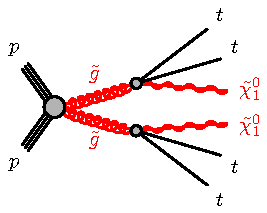
\includegraphics[width=\textwidth]{gogo-ttttN1N1}\caption{}\label{fig:feynman_gtt}\end{subfigure} &
\begin{subfigure}[t]{0.24\textwidth}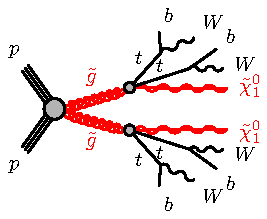
\includegraphics[width=\textwidth]{gogo-WWWWbbbbN1N1}\caption{}\label{fig:feynman_gttOffshell}\end{subfigure} &
\begin{subfigure}[t]{0.24\textwidth}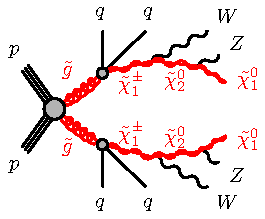
\includegraphics[width=\textwidth]{gogo-qqqqWWZZN1N1-C1N2}\caption{}\label{fig:feynman_gg2WZ}\end{subfigure} &
\begin{subfigure}[t]{0.24\textwidth}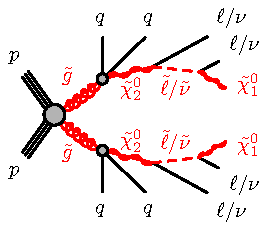
\includegraphics[width=\textwidth]{gogo-qqqqllllN1N1-N2}\caption{}\label{fig:feynman_gg2sl}\end{subfigure}  \\
\begin{subfigure}[t]{0.24\textwidth}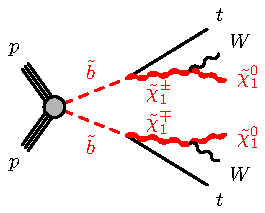
\includegraphics[width=\textwidth]{sbsb-ttWWN1N1}\caption{}\label{fig:feynman_b1b1}\end{subfigure} &
\begin{subfigure}[t]{0.24\textwidth}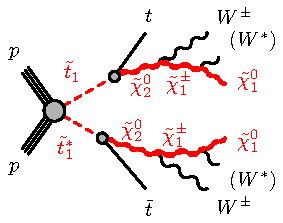
\includegraphics[width=\textwidth]{stst-ttWWWWN1N1}\caption{}\label{fig:feynman_t1t1}\end{subfigure} & 
\begin{subfigure}[t]{0.24\textwidth}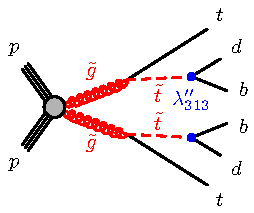
\includegraphics[width=\textwidth]{gogo-ttbbdd-stst-RPV}\caption{}\label{fig:feynm_rpv_gl313}\end{subfigure} &
\begin{subfigure}[t]{0.24\textwidth}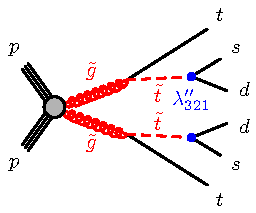
\includegraphics[width=\textwidth]{gogo-ttddss-stst-RPV}\caption{}\label{fig:feynm_rpv_gl321}\end{subfigure} \\
\begin{subfigure}[t]{0.24\textwidth}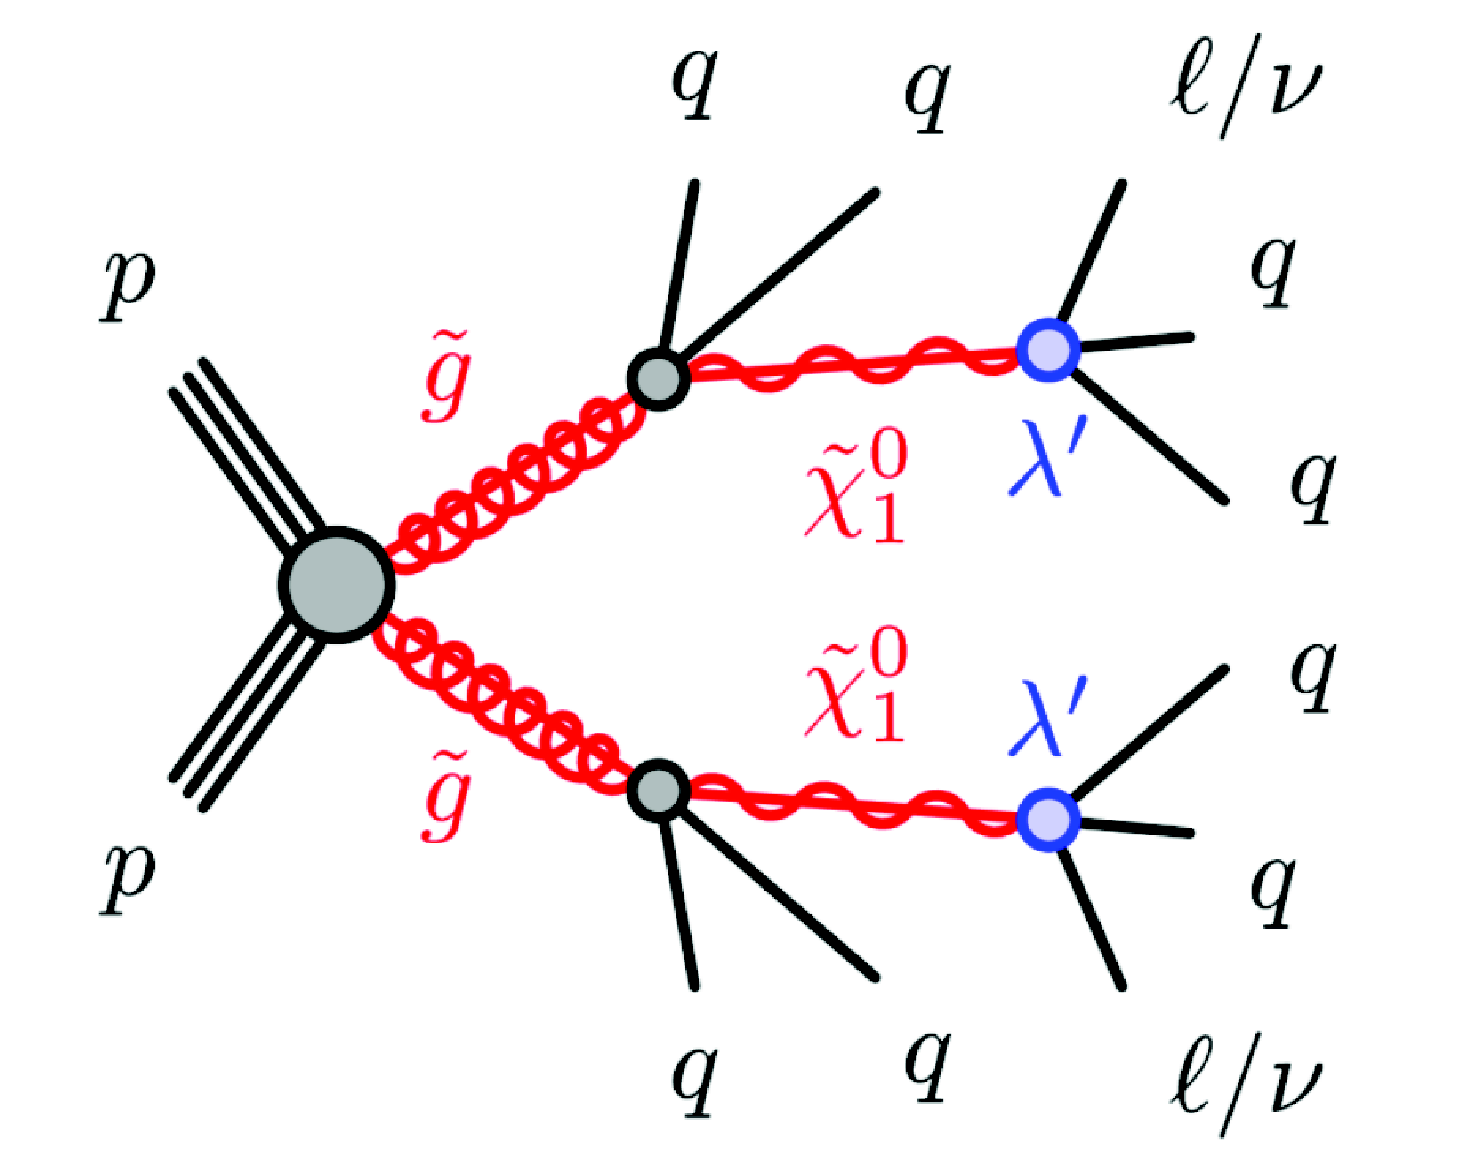
\includegraphics[width=\textwidth]{gogo-qqlqd-RPV}\caption{}\label{fig:feynm_rpv_glprime}\end{subfigure} & 
\begin{subfigure}[t]{0.24\textwidth}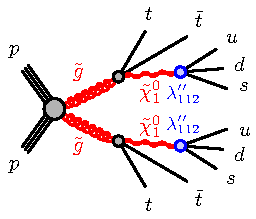
\includegraphics[width=\textwidth]{gogo-ttudd-RPV}\caption{}\label{fig:feynm_rpv_gl112}\end{subfigure} &
\begin{subfigure}[t]{0.24\textwidth}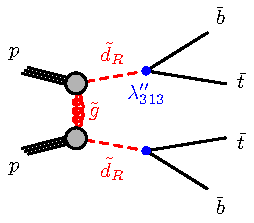
\includegraphics[width=\textwidth]{sdsd-ttbb-RPV}\caption{}\label{fig:feynm_rpv_sd313}\end{subfigure} &
\begin{subfigure}[t]{0.24\textwidth}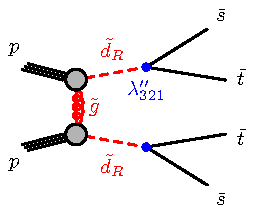
\includegraphics[width=\textwidth]{sdsd-ttss-RPV}\caption{}\label{fig:feynm_rpv_sd321}\end{subfigure} \\
\end{tabular}
\caption{RPC SUSY processes featuring gluino (a, b, c, d) or third generation squark (e, f) pair production studied in this analysis. 
RPV SUSY models considered are gluino pair production (g, h, i, j) and t-channel production of right-handed down squarks(k, l) which decay via baryon 
or lepton number violating couplings $\lambda''$ and $\lambda'$ respectively. In the diagrams, $q= u, d, c, s$ and $\ell=e,\mu,\tau$.}
\label{fig:feynman}
\end{figure}

In the case of non-zero RPV couplings in the baryonic sector ($\lambda''_{ijk}\neq 0$),
as proposed in minimal flavor violation scenarios~\cite{Nikolidakis:2007fc,Smith:2008ju,Csaki:2011ge},
gluino and squarks may decay directly to top quarks, leading to final states with same-sign leptons~\cite{Durieux:2013uqa,Berger:2013sir} 
and $b$-tagged jets (Figs.~\ref{fig:feynm_rpv_gl313},~\ref{fig:feynm_rpv_gl321}).
Alternatively a gluino decaying to a neutralino LSP, that further decays to SM particles via a non-zero $\lambda'$ or $\lambda''$ RPV coupling, 
is also possible (Figs.~\ref{fig:feynm_rpv_glprime},~\ref{fig:feynm_rpv_gl112}).  
Lower $\met$ is expected in these scenarios, as there is no stable LSP, and the only \met originates from neutrinos produced in the top quark decays.
Pair-production of right-handed\footnote{These RPV baryon-number-violating couplings only couple to $SU(2)$ singlets.} 
like-sign down squarks (Figs.~\ref{fig:feynm_rpv_sd313},~\ref{fig:feynm_rpv_sd321}) are also considered.
In all of these scenarios, antisquarks decay into the charge-conjugate final states of those indicated for the corresponding squarks, 
and gluinos decay with equal probabilities into the given final state or its charge conjugate.

After describing the experimental apparatus~(Section~\ref{sec:detector}) and
the simulated event samples~(Section~\ref{sec:dataMC}), the 19 signal regions (SRs) designed to achieve 
good sensitivity for the 12 SUSY scenarios of Fig.~\ref{fig:feynman} are presented (Section~\ref{sec:selection}).
Section~\ref{sec:bkg} describes the estimation of the contribution from SM processes to the signal regions, 
validated by comparisons with data in dedicated regions. Systematics are described in Section~\ref{sec:syst}. 
The results are presented in Section~\ref{sec:result} together with the statistical procedure used to interpret 
the results in the context of the SUSY benchmark scenarios. Finally, Section~\ref{sec:conclusion} summarises the main conclusions.

%-------------------------------------------------------------------------------
\section{The ATLAS detector}
\label{sec:detector}
%-------------------------------------------------------------------------------

The ATLAS experiment~\cite{PERF-2007-01} is a multi-purpose particle detector with a forward-backward symmetric cylindrical
geometry and nearly $4\pi$ coverage in solid angle.\footnote{ATLAS uses
  a right-handed coordinate system with its origin at the nominal
  interaction point (IP) in the centre of the detector and the
  $z$-axis along the beam pipe. The $x$-axis points from the IP to the
  centre of the LHC ring, and the $y$-axis points upward. Cylindrical
  coordinates ($r$, $\phi$) are used in the transverse plane, $\phi$
  being the azimuthal angle around the beam pipe. The pseudorapidity
  is defined in terms of the polar angle $\theta$ as $\eta = -\ln
  \tan(\theta/2)$. Rapidity is defined as $y=0.5 \ln\left[(E + p_z )/(E - p_z )\right]$ 
  where $E$ denotes the energy and $p_z$ is the component of the momentum along the beam direction. 
  The transverse momentum \pt, the transverse energy \et and the missing transverse momentum \met 
  are defined in the $x-y$ plane.}
The interaction point is surrounded by an inner detector (ID), a
calorimeter system, and a muon spectrometer (MS).

The ID provides precision tracking of charged particles with
pseudorapidities $|\eta| < 2.5$ and is surrounded by a superconducting solenoid providing a \SI{2}{T} axial magnetic field.
It consists of pixel and silicon-microstrip detectors inside a
transition radiation tracker. One significant upgrade for the $\sqrt{s}=13$~TeV running period is the presence of the
Insertable B-Layer~\cite{CERN-LHCC-2010-013}, an additional pixel layer close to the interaction point, which 
provides high-resolution hits at small radius to improve the tracking performance.

In the pseudorapidity region $|\eta| < 2.5$, high-granularity lead/liquid-argon 
electromagnetic sampling calorimeters are used.
A steel/scintillator tile calorimeter measures hadron energies for $|\eta| < 1.7$.
The endcap and forward regions, spanning $1.5<|\eta| <4.9$, are 
instrumented with liquid-argon calorimeters 
for both the electromagnetic and hadronic measurements. 

The MS consists of three large superconducting toroids
with eight coils each, 
a system of trigger and precision-tracking chambers, 
which provide triggering and tracking capabilities in the
ranges $|\eta| < 2.4$ and $|\eta| < 2.7$, respectively.

A two-level trigger system is used to select events~\cite{Aad:2012xs,ATL-DAQ-PUB-2016-001,Aaboud:2016leb}. The first-level
trigger is implemented in hardware. This is followed by the software-based High-Level Trigger stage,
which can run offline-like reconstruction, reducing the event rate to about \SI{1}{kHz}.



%-------------------------------------------------------------------------------
\section{Dataset and simulated event samples}
\label{sec:dataMC}
%-------------------------------------------------------------------------------

The data were collected by the ATLAS detector during 2015 and 2016 with a peak 
instantaneous luminosity of $L~=~1.4\times~10^{34}$~cm$^{-2}$s$^{-1}$. 
The mean number of $pp$ interactions per bunch crossing 
(pile-up) in the dataset is $\langle \mu \rangle = 23.7$ and
the bunch spacing is 25ns. After the application of beam, detector and data quality requirements, 
the integrated luminosity considered in this analysis corresponds to 36.0~fb$^{-1}$.
The preliminary uncertainty on the combined 2015+2016 integrated luminosity is 3.2\%. 
It is derived, following a methodology similar to that detailed in Ref.~\cite{Aaboud:2016hhf}, 
from a preliminary calibration of the luminosity scale using $x$-$y$ beam-separation scans performed in August 2015 and May 2016.

Monte Carlo (MC) simulated event samples are used to estimate the irreducible SM background with two 
same-sign and or three prompt leptons to model the SUSY signals. The reducible background, mainly 
coming from $\ttbar$ production, is estimated from the data as described in detail in Section~\ref{sec:bkg}. 
The MC samples are processed through an ATLAS detector simulation~\cite{Aad:2010ah} based on 
{\sc Geant4}~\cite{Agostinelli:2002hh} or a fast simulation using a parameterisation of the calorimeter response 
and {\sc Geant4} for the ID and MS~\cite{ATL-PHYS-PUB-2010-013}. To simulate the effects of additional $pp$ collisions 
in the same and nearby bunch crossings, additional interactions are generated using the soft QCD processes 
of \PYTHIA 8.186~\cite{Sjostrand:2007gs} with the A2 tune~\cite{ATLAS-PHYS-PUB-2012-003} and the MSTW2008LO PDF~\cite{Martin:2009iq}, 
and overlaid onto the simulated hard scatter event. 
The MC events are reweighted to match the pile-up conditions observed in the data and are reconstructed in the 
same manner as the data. The generator, parton shower, cross-section normalisation, parton distribution function (PDF) 
set and underlying-event tune of all samples are given in Table~\ref{tab:MC}.In all MC samples, except 
those produced by \SHERPA, the {\sc EvtGen}~v1.2.0 program~\cite{EvtGen} is used to model the properties 
of the bottom and charm hadron decays. 



\begin{table*}[ht]
\begin{center}
\scriptsize
\resizebox{\textwidth}{!}
{
\begin{tabular}{|l|l|c|c|c|c|}
\hline
Physics process    & Generator & Parton shower & Cross-section & PDF set & Tune \\
                   &	      & 	      & normalisation & 	&      \\
\hline
RPC signal 	   & \AMCATNLO 2.2.3~\cite{Alwall:2014hca} & \PYTHIA 8.186~\cite{Sjostrand:2007gs}&NLO+NLL~\cite{Beenakker:1996ch,Kulesza:2008jb,Kulesza:2009kq,Beenakker:2009ha,Beenakker:2011fu,Kramer:2012bx} & NNPDF2.3LO~\cite{Lai:2010vv} & A14~\cite{pub-2014-021} \\
        	   &  		           & 		       & or NLO-Prospino2 			& 			     &   \\
RPV signal 	   & \AMCATNLO 2.2.3        & \PYTHIA 8.210       & NLO+NLL or			 & NNPDF2.3LO		       & A14 \\
        	   &  		           & 		       & NLO-Prospino2 			& 			     &   \\
\hline
$\ttbar+W/Z/\gamma^{*}$ & \AMCATNLO 2.2.2 & \PYTHIA 8.186	  & NLO~\cite{YR4}     & NNPDF2.3LO & A14    \\
$\ttbar H$	   & \AMCATNLO 2.2.2        & \HERWIG 2.7.1~\cite{Corcella:2000bw}                & NLO~\cite{YR4}   &
CTEQ6L1~\cite{Pumplin:2002vw} & UEEE5~\cite{Gieseke:2012ft}  \\
$\ttbar\ttbar$     & \AMCATNLO 2.2.2       & \PYTHIA 8.186        & NLO~\cite{Alwall:2014hca}	  & NNPDF2.3LO	  & A14  \\
Diboson    & \SHERPA 2.1.1~\cite{gleisberg:2008ta}               & \SHERPA 2.1.1	& NLO~\cite{pubnote_mc_multiboson}	 &CT10~\cite{Lai:2010vv} & \SHERPA default \\
\hline
$\ttbar+WW/WZ$     & \AMCATNLO 2.2.2       & \PYTHIA 8.186         & NLO~\cite{Alwall:2014hca}	  & NNPDF2.3LO	  & A14  \\
$t+Z/WZ/\ttbar$    & \AMCATNLO 2.2.2        & \PYTHIA 8.186       & LO~\cite{YR4}                   	 & NNPDF2.3LO     & A14  \\
Triboson	   & \SHERPA 2.1.1         & \SHERPA 2.1.1        & LO, NLO~\cite{pubnote_mc_multiboson}            & CT10	     & \SHERPA default \\
$H+W/Z$	           & \AMCATNLO 2.2.2        & \PYTHIA 8.186       & NLO~\cite{Dittmaier:2012vm}   & NNPDF2.3LO     & A14  \\
\hline
\end{tabular}
}
\caption{Simulated signal and background event samples: the corresponding generator, parton shower, cross-section normalisation, PDF set and 
underlying-event tune are shown. Because of their very small contribution to the signal region background estimate 
$\ttbar+WW/WZ$, $t+Z/WZ/\ttbar$, $H+W/Z$ and triboson are summed and called ``Rare'' in the following. 
NLO-Prospino2 refers to RPV down squark models of Fig.\ref{fig:feynm_rpv_sd313} and \ref{fig:feynm_rpv_sd321}, as well as NUHM2.}
\label{tab:MC}
\end{center}
\end{table*}

The SUSY signals are defined by an effective Lagrangian describing the interactions of a small number of new 
particles~\cite{Alwall:2008ve,Alwall:2008ag,Alves:2011wf}. All SUSY particles not included 
in the decay of the pair-produced squarks and gluinos have their masses effectively decoupled. These models assume one 
production process and one decay channel with a 100\% branching fraction. They are generated 
from Leading Order (LO) matrix elements with up to two extra partons in the matrix element 
(only up to one for the $\gluino\to q\bar q(\ell\ell/\nu\nu)\neut$ model) 
using \AMCATNLO 2.2.3~\cite{Alwall:2014hca} interfaced to Pythia 8.186 with the A14 tune~\cite{pub-2014-021} for the 
modelling of the parton shower, hadronisation and underlying event.
Jet--parton matching is realised following the CKKW-L prescription~\cite{Lonnblad:2011xx}, with a matching scale set to one quarter of 
the pair-produced superpartner mass. The PDF set used for the generation is NNPDF23LO~\cite{Lai:2010vv}. All signal models are generated 
with prompt decays of the SUSY particles. Signal cross-sections are calculated to NLO in the strong coupling constant, 
adding the resummation of soft gluon emission at next-to-leading-logarithmic 
accuracy (NLO+NLL)~\cite{Beenakker:1996ch,Kulesza:2008jb,Kulesza:2009kq,Beenakker:2009ha,Beenakker:2011fu}, except 
for the RPV models of Fig.\ref{fig:feynm_rpv_sd313} and Fig.\ref{fig:feynm_rpv_sd321} as well as the NUHM2 model where NLO 
cross-sections are used~\cite{Beenakker:1996ed,Beenakker:1996ch}. The nominal cross-sections and the uncertainties are taken from 
envelopes of cross-section predictions using different PDF sets 
and factorisation and renormalisation scales, as described in Ref.~\cite{Kramer:2012bx}. 
Typical production cross-sections are: $(4.7 \pm 1.2)$~fb for gluino pairs with a mass of \SI{1.7}{\TeV}, $(28.3 \pm 4.0)$~fb
for bottom squark pairs with a mass of \SI{800}{\GeV}, and $(15.0\pm 2.0)$~fb for right-handed down 
squark pairs with a mass of \SI{800}{\GeV} and a gluino mass of \SI{2.0}{\TeV}.

The two dominant background processes are $\ttbar V$ (with $V=W$ and $Z$, including non-resonant $Z/\gamma^*$ contributions) 
and diboson with four charged leptons ($\ell$ including here all lepton flavors, where $\tau$
leptons subsequently can decay leptonically or hadronically), three charged leptons and one neutrino, or 
two same-sign charged leptons and two neutrinos. They are described in details in Refs.~\cite{pubnote_mc_ttv} and~\cite{pubnote_mc_multiboson}, 
respectively. Samples of the former are generated with one ($\ttbar Z$) and two ($\ttbar W$) extra partons. Similarly for the latter, 
one ($W^\pm W^\pm jj$) and two ($WZ$, $ZZ$) extra partons are simulated. NLO cross-sections for 
$\ttbar W$, $\ttbar Z/\gamma^*(\rightarrow \ell \ell)$ and dibosons are respectively 600.8~fb~\cite{YR4}, 
123.7~fb\footnote{This cross-section is computed using the configuration of Refs.~\cite{Alwall:2014hca,Frixione:2015zaa}.} and 
40.0~pb~\cite{pubnote_mc_multiboson}. The processes $\ttbar H$ and $\ttbar \ttbar$, with NLO cross-sections of 507.1~fb~\cite{YR4} and 
9.2~fb~\cite{Alwall:2014hca} respectively, are also considered.

Other low cross-section background processes are grouped into ``Rare'' in the following. This category contains 
samples of $\ttbar+WW/WZ$ with no extra parton in the matrix element, $t+Z/WZ/\ttbar$, $H+W/Z$ as well as 
triboson ($WWW$, $WWZ$, $WZZ$ and $ZZZ$) production with up to six charged leptons. The $4\ell$ and $2\ell+2\nu$ processes are 
calculated at NLO with up to one additional parton; final states with two and three additional partons are calculated at leading order (LO). 
The $WWZ\to 4\ell+2\nu$ or $2\ell+4\nu$ processes are calculated at LO with up to two additional partons. 
The $3\ell +1\nu$ process is calculated at NLO with up to three extra partons at LO using the Comix~\cite{Gleisberg:2008fv} 
and OpenLoops~\cite{Cascioli:2011va} matrix element generators and merged with the \SHERPA~\cite{Schumann:2007mg} 
using the ME+PS@NLO prescription for the parton shower~\cite{Hoeche:2012yf}. The $WWZ/WZZ\to 3\ell+3\nu$, $ZZZ\to 6\ell+0\nu$, $4\ell+2\nu$ or $2\ell+4\nu$ processes 
are calculated with the same configuration but with up to only two extra partons at LO.


%-------------------------------------------------------------------------------
\section{Event selection}
\label{sec:selection}
%-------------------------------------------------------------------------------

Candidate events are required to have a reconstructed vertex~\cite{ATL-PHYS-PUB-2015-026}, 
with at least two associated tracks with $\pt >400$~MeV, 
and the vertex with the highest sum of squared transverse 
momentum of the tracks is considered as primary vertex.
In order to perform background estimations using data, 
two categories of electrons and muons are defined: 
``candidate'' and ``signal'' (the latter being a subset of the ``candidate'' leptons satisfying tighter selection criteria). 

Electron candidates are reconstructed from an isolated electromagnetic 
calorimeter energy deposit matched to an ID track and are required to have $|\eta|<2.47$, 
a transverse momentum $\pT>\SI{10}{\GeV}$, 
and to pass a loose likelihood-based identification requirement~\cite{elecperf,ATL-PHYS-PUB-2015-041}. 
The likelihood input variables include measurements of calorimeter shower shapes and measurements of track properties from the ID. 
Candidates within the transition region between the barrel and endcap electromagnetic calorimeters,
$1.37<|\eta|<1.52$, are removed. 
The track matched with the electron must have a significance of the transverse impact parameter 
with respect to the reconstructed primary vertex, $d_0$, of $\vert d_0\vert/\sigma(d_0) < 5$.

Muon candidates are reconstructed in the region $|\eta|<2.5$ 
from muon spectrometer tracks matching ID tracks.
All muons must have $\pT>\SI{10}{\GeV}$ and must pass the medium identification requirements defined in Ref.~\cite{Run2Muon}, 
based on selections on the number of hits in the different ID and muon spectrometer subsystems, 
and the significance of the charge to momentum ratio $q/p$~\cite{Run2Muon}.

Jets are reconstructed with the anti-$k_t$
algorithm~\cite{Cacciari:2008} with radius parameter $R=0.4$, using three-dimensional energy
clusters in the calorimeter~\cite{caloclusters} as input. 
All jets must have $\pT>\SI{20}{\GeV}$ and $|\eta|<2.8$.
Jets are calibrated as described in Ref.~\cite{ATLAS-PHYS-PUB-2015-015}.
In order to reduce the effects of pile-up, 
for jets with $\pt<\SI{50}{GeV}$ and $|\eta|<2.4$ a significant fraction of the tracks associated with each jet
must have an origin compatible with the primary vertex, 
as defined by the jet vertex tagger~\cite{ATLAS-CONF-2014-018}. 
Furthermore, for all jets the expected average energy contribution from
pile-up clusters is subtracted according to the jet area~\cite{ATLAS-PHYS-PUB-2015-015}.

Identification of jets containing $b$-hadrons ($b$-tagging) is performed with the MV2c20 algorithm, 
a multivariate discriminant making use of track impact parameters 
and reconstructed secondary vertices~\cite{Aad:2015ydr,ATL-PHYS-PUB-2015-022}.
A requirement is chosen corresponding to a 70\% average efficiency 
obtained for $b$-jets in simulated $\ttbar$ events. 
The rejection factors for light-quark jets, $c$-quark jets and hadronically decaying $\tau$ leptons in simulated $\ttbar$ events 
are approximately 440, 8 and 26, respectively~\cite{ATL-PHYS-PUB-2015-022}. 
Jets with $|\eta|<2.5$ which satisfy this $b$-tagging requirement are identified as $b$-jets. 
To compensate for differences between data and MC simulation in the $b$-tagging efficiencies and mis-tag rates, 
correction factors are applied to the simulated samples~\cite{ATL-PHYS-PUB-2015-022}. 

After object identification, overlaps between objects are resolved. 
Any jet within a distance $\Delta R_y =\sqrt{(\Delta y)^2+(\Delta\phi)^2}$ = 0.2 of an electron candidate is discarded, 
unless the jet has a value of the MV2c20 discriminant larger than the value corresponding to approximately an 80\% $b$-tagging efficiency, 
in which case the electron is discarded since it is likely originating from a semileptonic $b$-hadron decay. 
Any remaining electron within $\Delta R_y=$ 0.4 of a jet is discarded. 
Muons within $\Delta R_y=$ 0.4 of a jet are also removed. 
However, if the jet has fewer than three associated tracks, the muon is kept and the jet is discarded instead 
to avoid inefficiencies for high-energy muons undergoing significant energy loss in the calorimeter.

Signal electrons must satisfy a tight likelihood-based identification requirement~\cite{elecperf,ATL-PHYS-PUB-2015-041} 
and have $|\eta|<2$ to reduce the impact of electron charge mis-identification. 
Signal muons must fulfil the requirement of $\vert d_0\vert/\sigma(d_0) < 3$. 
The track associated to the signal leptons must have a longitudinal impact parameter with respect to the reconstructed primary vertex, $z_0$, 
satisfying $\vert z_0 \sin\theta\vert  < 0.5$~mm. 
Isolation requirements are applied to both the signal electrons and muons. 
The  scalar sum of the \pt of tracks within a variable-size cone around the lepton, 
excluding its own track, must be less than 6\% of the lepton \pt. 
The track isolation cone radius for electrons (muons) 
$\Delta R_\eta=\sqrt{(\Delta\eta)^2+(\Delta\phi)^2}$ 
is given by 
the smaller of $\Delta R_\eta = \SI{10}{~GeV}/\pt$ and $\Delta R_\eta = 0.2\,(0.3)$, 
that is, a cone of size $0.2\,(0.3)$ at low $\pt$ but narrower for high-\pt leptons. 
In addition, in the case of electrons the energy of calorimeter energy clusters in a cone of $\Delta R_\eta = 0.2$ around the electron 
(excluding the deposition from the electron itself) must be less than 6\% of the electron \pt. 
Simulated events are corrected to account for minor differences in the lepton trigger, reconstruction and 
identification efficiencies between data and MC simulation.

The missing transverse momentum ${\vec p}^{\rm miss}_{\rm T}$ is defined as the negative vector sum of the transverse momenta of all identified physics objects (electrons, photons, muons, jets) and an additional soft term. The soft term is constructed from all tracks that are not associated with any physics object, and that are associated with the primary vertex. In this way, the $\met$ is adjusted for the best calibration of the jets and the other identified physics objects above, while maintaining pile-up independence in the soft term~\cite{ATL-PHYS-PUB-2015-027, ATL-PHYS-PUB-2015-023}.

Events are selected using a combination (logical OR) of dilepton and $\met$ triggers, 
the latter being used only for events with $\met>\SI{250}{GeV}$. 
The trigger-level requirements on $\met$ and the leading and subleading lepton \pt are looser than those applied offline 
to ensure that trigger efficiencies are constant in the relevant phase space. 
Events of interest are selected if they contain at least two signal leptons with $\pt>20$~\GeV . 
If the event contains exactly two signal leptons, they are required to have the same electric charge. 

To maximise the sensitivity in different signal models, 
four overlapping signal regions are defined as shown in Table~\ref{tab:SRdef3}, with requirements on the number of signal leptons ($N_{\rm{lept}}^{\rm{signal}}$), 
the number of $b$-jets with $\pt>\SI{20}{\GeV}$ ($N_{b\rm{-jets}}^{20}$), 
the number of jets with $\pt>\SI{50}{\GeV}$ regardless of their flavour ($N_{\rm{jets}}^{50}$), 
\met\ 
and the effective mass (\meff), defined as the scalar sum of the $\pt$ of the signal leptons and jets (regardless of their flavour) in the event plus the \met. 

\begin{table}[tbh!]
\caption{Summary of the event selection criteria for the signal regions (see text for details).}
\hspace{0.5cm}
\def\arraystretch{1.3}
\label{tab:SRdef3}
\centering
\begin{tabular}{c|c|c|c|c|c}
\hline 
\hline
Signal region  &  $N_{\rm{lept}}^{\rm{signal}}$   & $N_{b\rm{-jets}}^{20}$    & $N_{\rm{jets}}^{50}$  & \met\ [GeV] & \meff\ [GeV]   \\
\hline\hline
SR0b3j &  $\ge$3  &    $=$0 &  $\ge$3 &  $>$200 & $>$550 \\
SR0b5j &  $\ge$2  &    $=$0 &  $\ge$5 &  $>$125 & $>$650 \\
SR1b     &  $\ge$2  &    $\ge$1  &  $\ge$4 &  $>$150 & $>$550 \\
SR3b     &   $\ge$2  &   $\ge$3  &  - & $>$125 & $>$650   \\
\hline\hline
\end{tabular}
\end{table}

Each signal region is motivated by a different SUSY scenario. 
The SR0b3j and SR0b5j signal regions are sensitive to gluino-mediated and directly produced squarks of the first and second generations 
leading to final states particularly rich in leptons (Fig.~\ref{fig:feynman_gg2sl}) or in jets (Fig.~\ref{fig:feynman_gg2WZ}), 
but with no enhancement of the production of $b$-quarks. 
Third-generation squark models resulting in final states with two $b$-quarks, 
such as direct bottom squark production (Fig.~\ref{fig:feynman_b1b1}), are targeted by the SR1b signal region. 
Finally, the signal region SR3b targets gluino-mediated top squark production resulting in final states with four $b$-quarks (Fig.~\ref{fig:feynman_gtt}).

The values of acceptance times efficiency of the SR selections for the SUSY signal models 
in Fig.~\ref{fig:feynman} typically range between 1\% and 6\% for $m_{\gluino}=\SI{1.2}{TeV}$ or $m_{\sbottomone}=\SI{600}{GeV}$, and a light \ninoone.


%-------------------------------------------------------------------------------
\section{Background estimation}
\label{sec:bkg}
%-------------------------------------------------------------------------------

Two main sources of SM background can be distinguished in this analysis. 
The first category is the reducible or detector background which includes 
events containing electrons with mis-measured charge, mainly from the production of top quark pairs, and events 
containing at least one non-prompt or fake lepton (FNP), which mainly originate from hadron decays in events containing 
top quarks, $W$ or $Z$ bosons. Data-driven methods used for the estimation
of this background are described in Section~\ref{sec:DD_bkg}. The second category consists of events 
with two same-sign prompt leptons or at least three prompt leptons and is 
estimated using the MC samples described in Section~\ref{sec:dataMC}. 
Since diboson and $\ttbar V$ events are the main backgrounds in the signal regions, 
dedicated validation regions (VR) with an enhanced contribution from these processes 
are defined to verify the background predictions from the simulation (see Section~\ref{sec:valid}).


\subsection{Detector background estimation methods} 
\label{sec:DD_bkg}

Background events due to charge mis-identification concerns only the electron. The probability of mis-identifying the 
charge of a muon is checked in both data and MC simulation, and found to be negligible in the kinematic range relevant to this analysis.
The contribution of charge-flip events to the SR/VR yields is estimated using the data. 
The electron charge-flip probability is extracted in a $Z/\gamma^{*}\to ee$ data sample using a likelihood fit 
which takes as input the numbers of same-sign and opposite-sign electron pairs observed in a window around the $Z$ mass. 
The charge-flip probability is a free parameter of the fit and is extracted as a function of the electron $\pt$ and $\eta$. 
These probabilities are in the range \textcolor{red}{UPDATE:1--5\%} and \textcolor{red}{UPDATE:0.1--1\%} for the candidate 
and signal electrons respectively.
The event yield of this background in the signal or validation regions is obtained by applying the measured charge-flip probability 
to the data regions with the same kinematic requirements as the signal or validation regions but with opposite-sign lepton pairs. 

The contribution from fake or non-prompt leptons (such as hadrons mis-identified as leptons, 
leptons originating from heavy-flavour decays, and electrons from photon conversions) 
is also estimated from the data with a matrix method similar to that described in Ref.~\cite{SUSY3bjetsRun1}. 
In this method, two types of lepton identification criteria are defined: ``tight'', 
corresponding to the signal lepton criteria described in Section~\ref{sec:selection}, 
and ``loose'', corresponding to candidate leptons after overlap removal. 
The matrix method relates the number of events containing prompt or FNP leptons 
to the number of observed events with tight or loose-not-tight leptons 
using the probability for loose prompt or FNP leptons to satisfy the tight criteria. 
The probability for loose prompt leptons to satisfy the tight selection criteria ($\epsilon$)
is obtained using a $Z/\gamma^*\to\ell\ell$ data sample 
and is modelled as a function of the lepton $\pt$ and $\eta$. 
The probability for loose FNP leptons to satisfy the tight selection criteria (FNP fake rate, $f$) is determined from data 
in SS and three lepton control regions enriched in non-prompt leptons originating from heavy-flavour decays, mostly coming from 
semileptonic $\ttbar$ events. This region contains events with at least one $b$-jet, 
one well-isolated ``tag'' muon, and an additional loose electron or muon on which the measurement is performed. 
The efficiencies are measured as function of \pt ($\eta$ binning is also used for low \pt muons) 
after subtracting the small contribution from prompt lepton processes. 

\textcolor{red}{[UPDATE: rewrite/inflate this paragraph]}The estimated FNP yields in the SRs are consistent with those 
predicted by two alternative methods: the first one relies on MC simulation of processes with FNP leptons or charge-flipped electrons 
($\ttbar$, $V$+jets)~\cite{paperSS3L,ATLAS-CONF-2012-151}, 
corrected to match the observed data in dedicated control regions. 
The second method relies on data events with only one lepton, which are the processes leading to FNP leptons, 
to extrapolate from low-\met\ control regions to the SRs.

%The data-driven background estimates are cross-checked with an MC-based technique. 
%In this method, the contributions from processes with FNP leptons and electron charge mis-identification 
%are obtained from MC simulation and normalised to data in dedicated control regions at low jet multiplicity, low $\met$, and 
%either with or without $b$-jets. 
%The normalisation is performed using five multipliers: one to correct 
%the electron charge mis-identification rate, and four to correct the contributions from FNP 
%electrons or muons originating from $b$-jets or light-flavour jets, respectively.
%In addition to the MC samples listed in Section~\ref{sec:dataMC}, this method employs samples of top quark pair production generated with the \POWHEG-Box v2 generator interfaced to \PYTHIA 6.428~\cite{Sjostrand:2006za}, 
%as well as samples of simulated $W$+jets and $Z$+jets events generated with \POWHEG-Box v2 interfaced to \PYTHIA 8.186.

% not the best place, but otherwise it's not well positionned wrt the text...
\begin{figure}[th!]
\centering
\begin{subfigure}[t]{0.49\textwidth}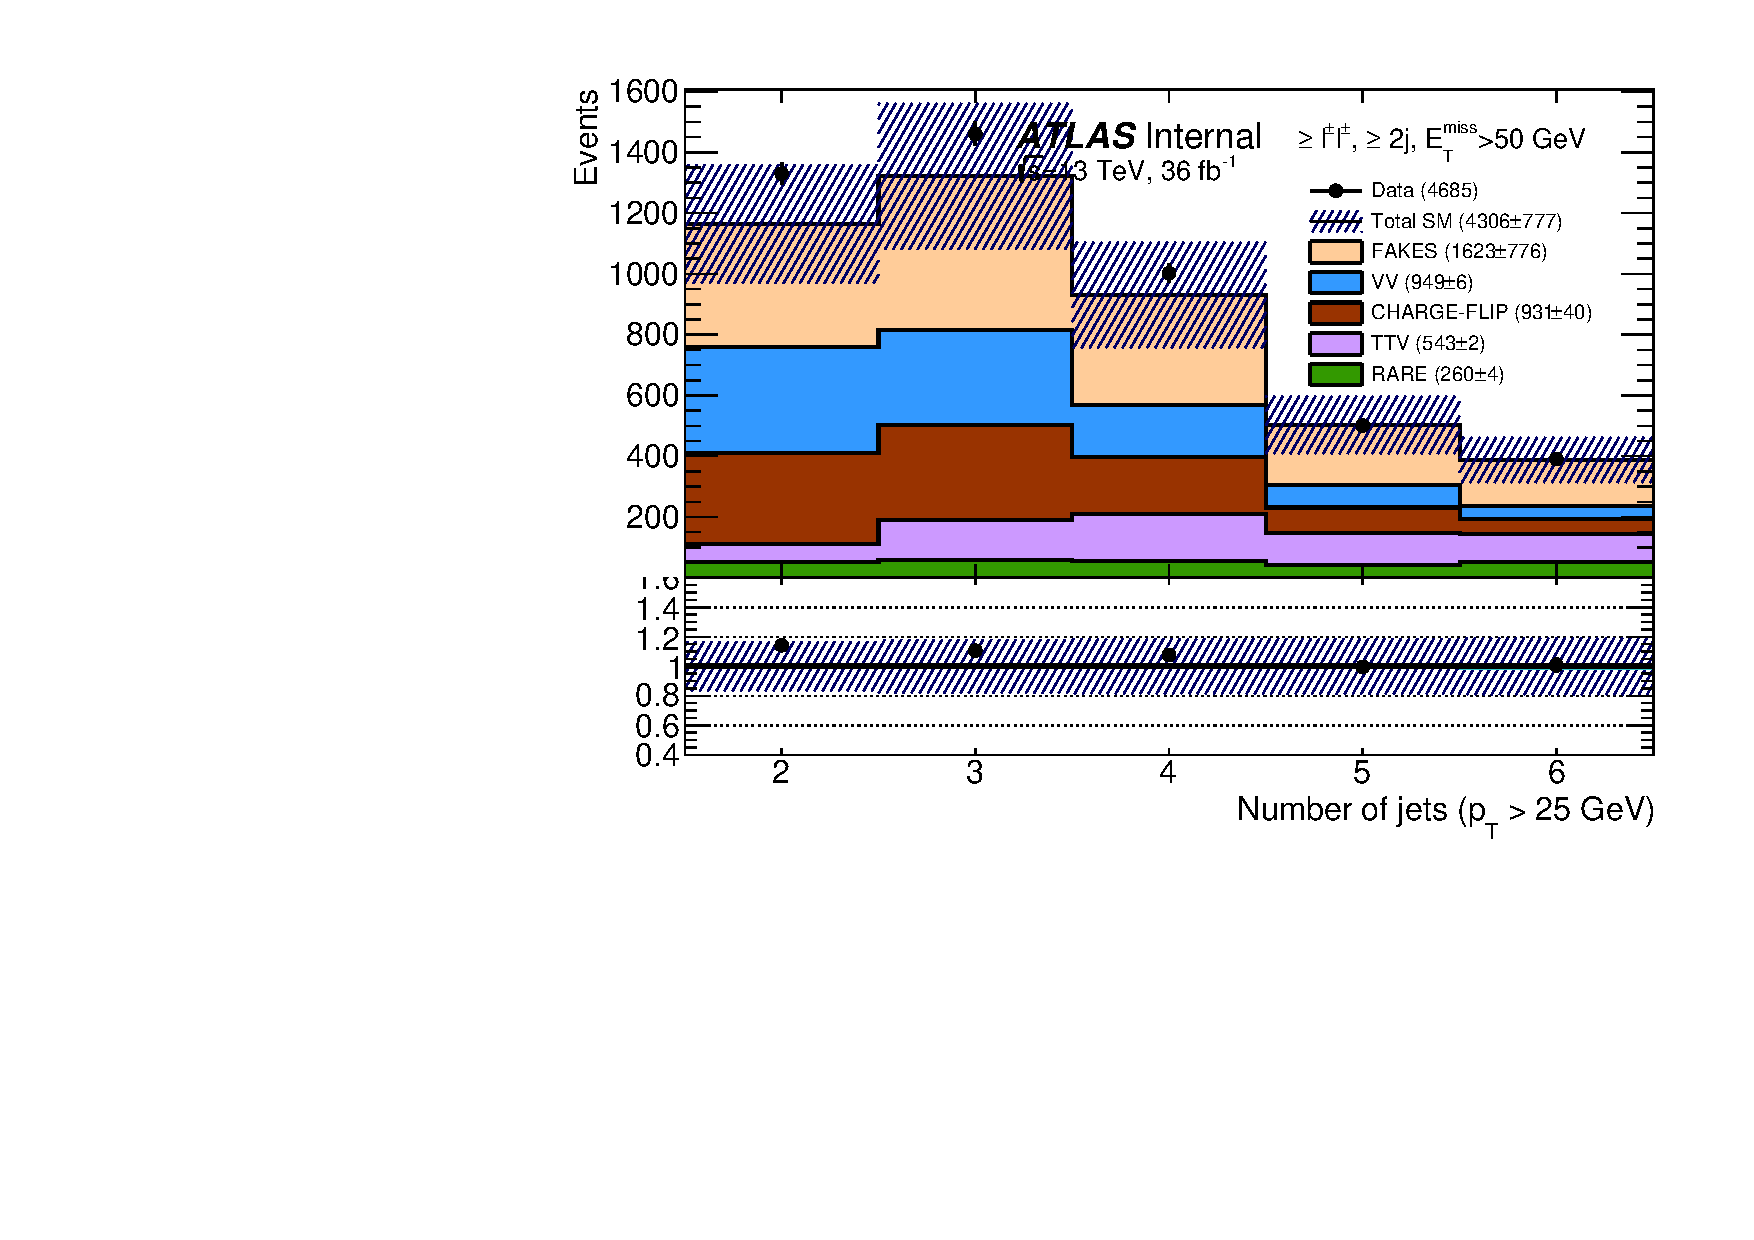
\includegraphics[width=\textwidth]{DILEP_2JMET50_njets25}\caption{}\end{subfigure}
\begin{subfigure}[t]{0.49\textwidth}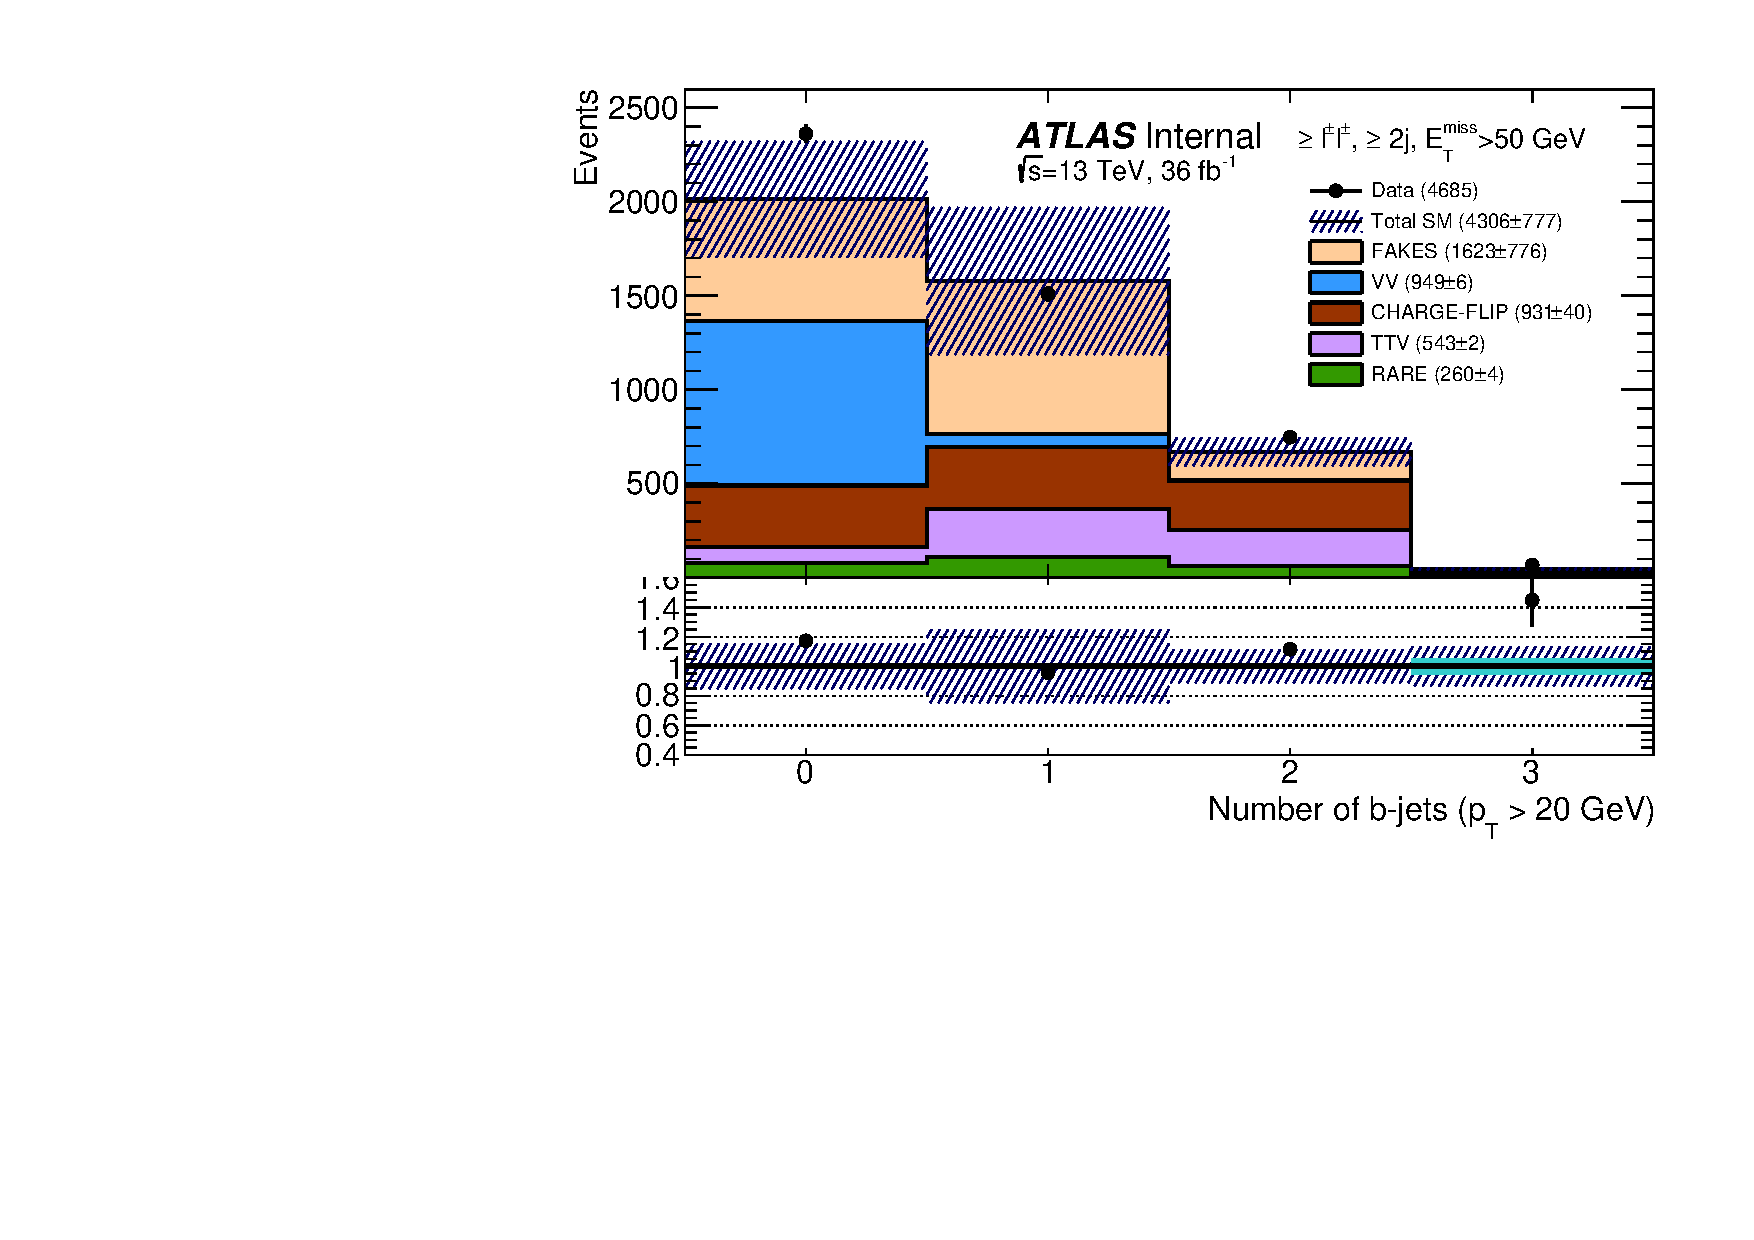
\includegraphics[width=\textwidth]{DILEP_2JMET50_nbjets}\caption{}\end{subfigure}
\begin{subfigure}[t]{0.49\textwidth}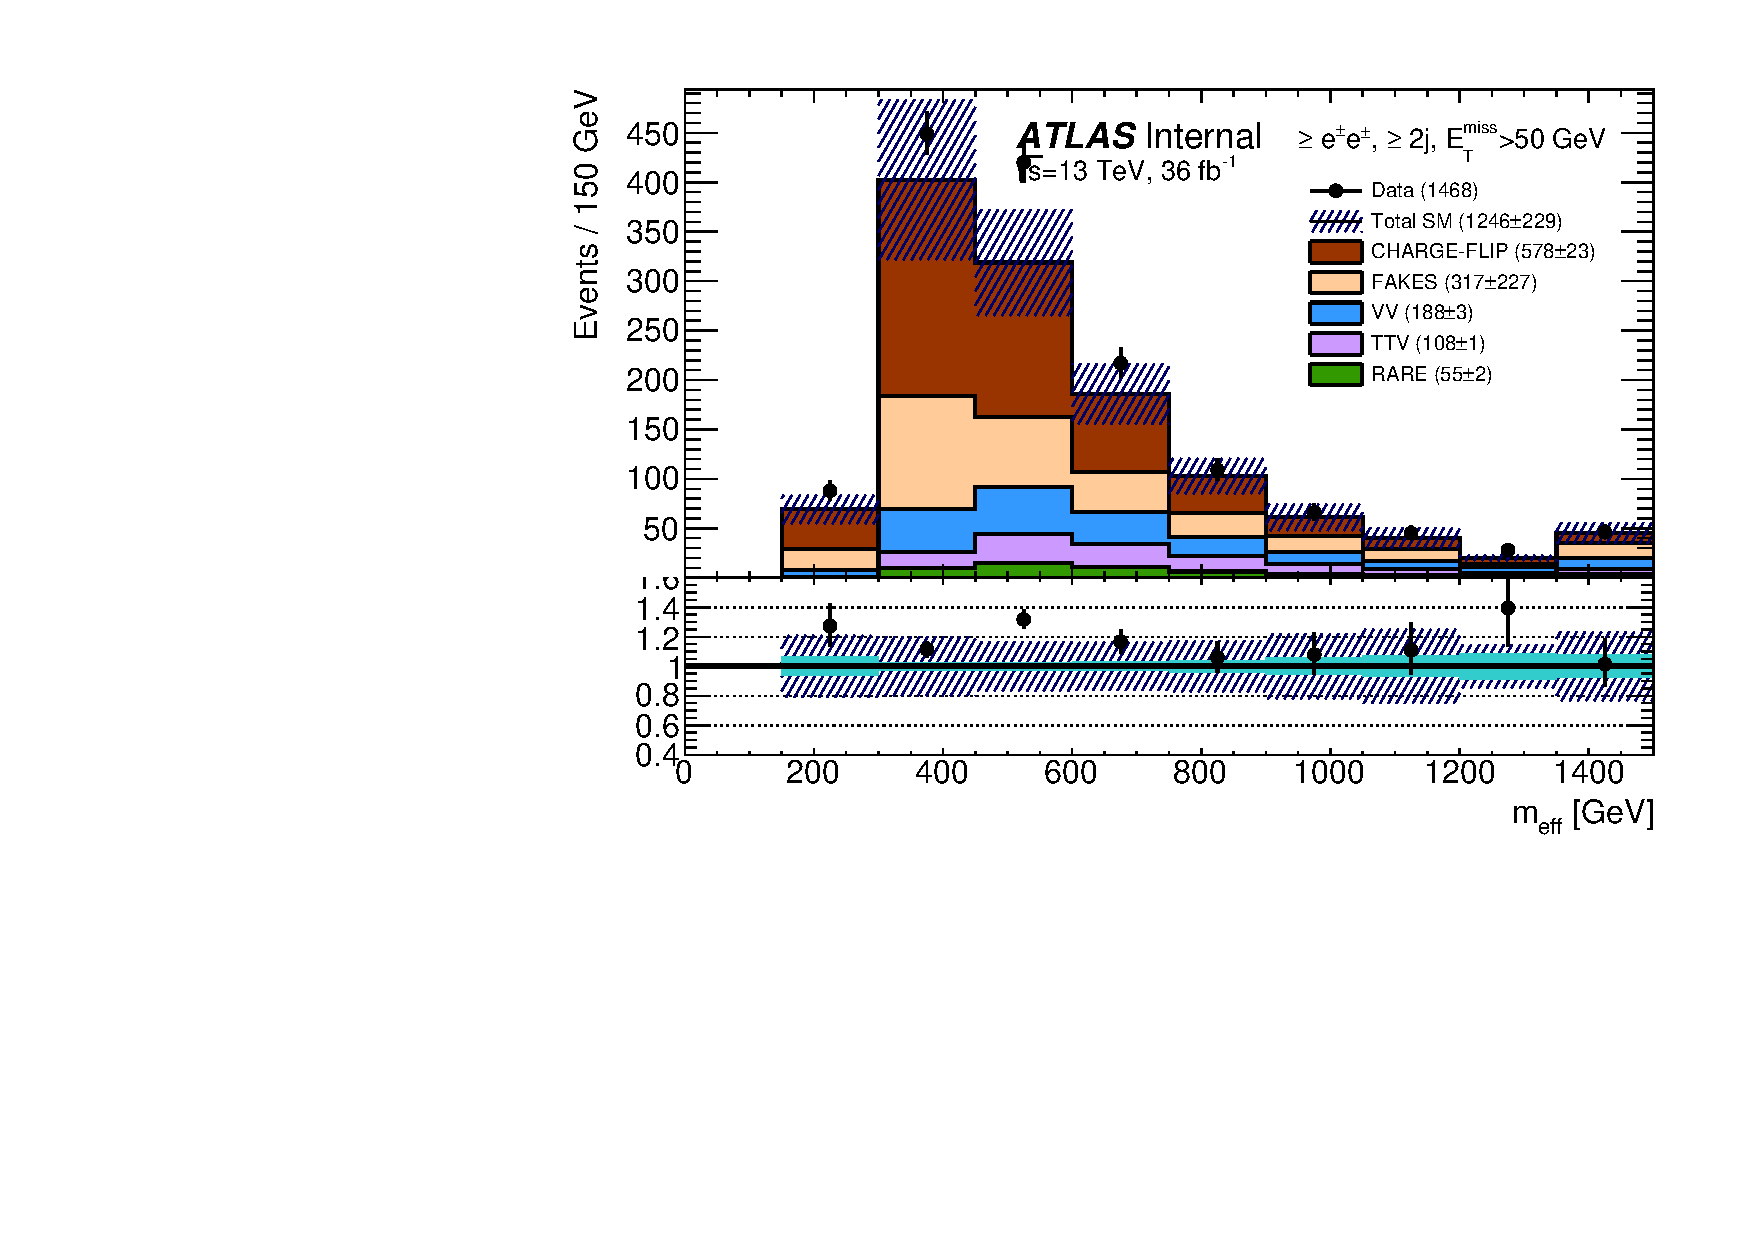
\includegraphics[width=\textwidth]{EE_2JMET50_meff}\caption{}\end{subfigure}
\begin{subfigure}[t]{0.49\textwidth}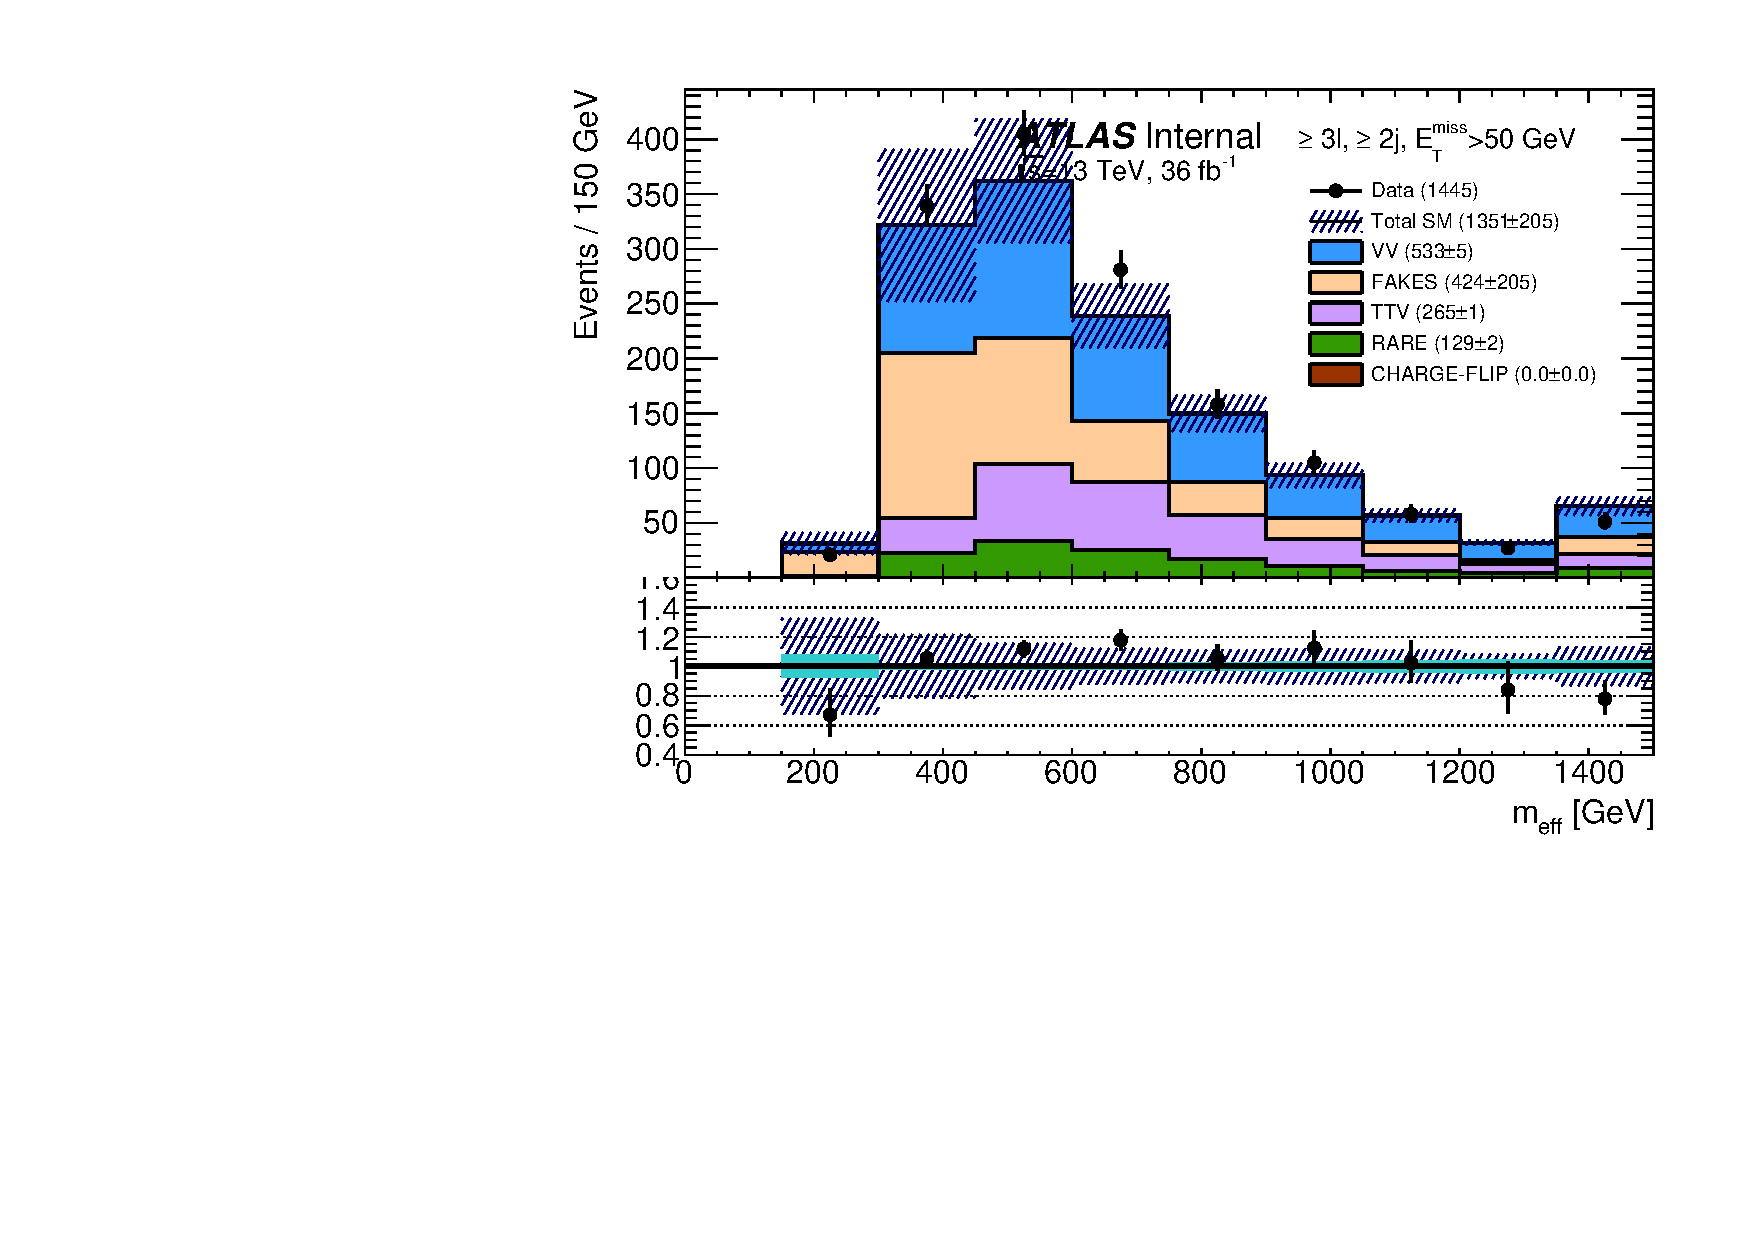
\includegraphics[width=\textwidth]{TRILEP_2JMET50_meff}\caption{}\end{subfigure}
\caption{
Distributions of the number of jets, of $b$-tagged jets and the effective mass after requiring at least two jets ($\pT>\SI{25}{GeV}$) and $\met>\SI{50}{GeV}$, 
as well as at least two same-sign leptons (a,b) or two same-sign electrons (c) or three leptons (d). 
The statistical uncertainties in the background prediction are included in the uncertainty band, 
as well as the full systematic uncertainties for backgrounds with fake or non-prompt leptons, or charge-flip. 
The light blue bands in the ratio plots show contributions from statistical uncertainties alone while the hashed area shows the total uncertainty.. 
The ``Rare'' category contains the contributions from associated production $\ttbar+WW/WZ$, 
as well as $t+Z/WZ/\ttbar$, $H+W/Z$, and triboson production. \textcolor{red}{[UPDATE: Remove numbers in the legend 
and move from upper case to lower case.]}
}
\label{fig:Bkg_distribs} 
\end{figure} 


\subsection{Validation of background estimates}
\label{sec:valid}

To check the validity and robustness of the background estimates, 
the distributions of several discriminating variables in data are compared 
with the predicted background after various requirements on the number of jets and $b$-jets. 
%Events are categorised based on the flavours of the selected leptons, and the different flavour channels are compared separately. 
Examples of such distributions are shown in Fig.~\ref{fig:Bkg_distribs}, 
and illustrate that the predictions and data agree fairly well. 

Dedicated validation regions are defined to test the estimate of the $\ttbar V$, $WZ$ and $W^\pm W^\pm$ SM processes contributing to the signal regions. The corresponding selections are summarized in Table~\ref{tab:VRdef}. 
In these regions, the overlap with the signal regions is resolved by vetoing events that contribute to the signal regions.  
%To further reduce contributions from electron charge mis-identification,  events are also vetoed in VR-$\ttbar W$ and VR-$W^\pm W^{\pm}jj$ if one of the two leading leptons is an electron with $|\eta|>1.37$\textcolor{red}{[UPDATE:Still true]}, since contributions from charge-flip electrons are smaller in the central region due to the lower amount of detector material in front of the calorimeters. 
The purity of the targeted processes in these regions ranges from about \textcolor{red}{[UPDATE:20\% to $50\%$]}. 

The observed yields in these validation regions, compared with the background predictions and uncertainties, 
can be seen in Table~\ref{tab:VR_yields}.
%, and the effective mass distributions are shown in Fig.~\ref{fig:VRd}--\ref{fig:VRf}.
There is good agreement between data and the estimated background for the validation regions.

\begin{table}[t!]
\hspace{0.5cm}
\def\arraystretch{1.1}
\centering
\resizebox{\textwidth}{!}
{\small
\begin{tabular}{|c|c|c|c|c|c|c|l|}
\hline    
Validation        &  $N_{\rm{lepton}}^{\rm{signal}}$ ($N_{\rm{lepton}}^{\rm{cand}}$)   & $N_{b\rm{-jets}}$  &  $N_{\rm{jets}}$  & $p^{}_{\rm{T,jet}}$  & \met\ & \meff\  & Other \\
Region Name       &  &  &  & [GeV]  & [GeV] & [GeV]  & \\
\hline\hline
$W^{\pm} W^{\pm}jj$ & $=2$ ($=2$)    &  $=0$ & $\geq 2$ &   $>50$ & $> 55$  & $> 650$ & veto $81<\mee<101$~GeV  \\
               	  & $=1$ SS pair  &	  &	     &         &   	&	  & $\pt^{\ell_2}>30$~GeV \\
               	  &		  &	  &	     &         &   	&	  & min$\left\{\Delta R(\ell_{1,2},j)\right\}>0.7$ \\
               	  &		  &	  &	     &         &   	&	  & min$\left\{\Delta R(\ell_1, \ell_2)\right\}>1.3$ \\
\hline
$WZ$4j            & $=3$ ($=3$)    &  $=0$ & $\geq 4$ &  $>25$   & --    & $> 450$ & $\met/\sum p_T^{\ell} < 0.7$ \\
\hline
$WZ$5j            & $=3$ ($=3$)    &  $=0$ & $\geq 5$ &  $>25$   & --    & $> 450$ & $\met/\sum p_T^{\ell} < 0.7$  \\ 
\hline
$\ttbar W$   	&$=2$ ($=2$)    &$\geq 1$   & $\geq 4$ ($e^\pm e^\pm$, $e^\pm \mu^\pm$) & $>40$ & $> 45$  & $> 550$   & $\pt(\ell_2)>40$~GeV\\
              	& $=1$ SS pair  &       &  $\geq 3$ ($\mu^\pm \mu^\pm$)   &  $>25$ &      &          & $\sum p_T^{b-jet}/\sum p_T^{jet}>0.25$ \\ 
\hline
$\ttbar Z$    	&$\geq 3$ (-) & $\geq 1$ & $\geq 3$ &  $>35$ &  --    & $> 450$  & $81<m_\text{SFOS}<101$~GeV \\
                &$\geq 1$ SFOS pair&     &          &       &         &         &  \\
\hline
All VRs & \multicolumn{7}{c|}{Veto events belonging to any SR} \\
\hline
\end{tabular}
}
\caption{Summary of the event selection in the validation regions (VRs). 
Requirements are placed on the number of signal leptons ($N_{\rm{lept}}^{\rm{signal}}$) 
and candidate leptons ($N_{\rm{lept}}^{\rm{cand}}$), the number of jets ($N_{\rm{jets}}$) 
or the number of $b$-jets with $\pt>\SI{20}{GeV}$ ($N_{b\rm{-jets}}$). The two leading-\pt 
leptons are referred to as $\ell_{1,2}$ with decreasing \pt. Additional requirements are set 
on \met, \meff, the invariant mass of the two leading electrons $m_{ee}$, the presence of SS 
leptons or a pair of same-flavour opposite-sign leptons (SFOS) and its invariant mass $m_\text{SFOS}$. 
A minimum angular separation between the leptons and the jets ($\Delta R (\ell, j)$) and between the two 
leptons ($\Delta R (\ell_{1}, \ell_2)$) is imposed in $W^\pm W^\pm$ VR. For the two $WZ$ VRs an upper cut 
on the ratio between the \met in the event and the sum of all selected leptons \pt (\met/$\sum{p_T^\ell}$) is required. 
An upper cut on the ratio between the sum of the \pt of all $b$-jets and that of all jets in the event ($\sum p_T^{b-j} / \sum{p_T^{j}}$) is 
considered only in the $\ttbar W$ VR.
}
\label{tab:VRdef}
\end{table}

\begin{table}[t!]
\hspace{0.5cm}
\def\arraystretch{1.1}
\centering
%\resizebox{\textwidth}{!}
%{\small
\begin{tabular}{|l|c|c|c|c|c|}
\hline    
 Validation Regions       & $WZ$4j & $WZ$5j  & $W^\pm W^{\pm}jj$& $\ttbar W$   & $\ttbar Z$  \\
\hline\hline
$t\bar{t}Z/\gamma^*$     & $  \pm  $ & $  \pm  $      & $  \pm  $  & $  \pm  $    & $  \pm  $  \\
$t\bar{t}W$              & $  \pm $  & $  \pm  $      & $  \pm  $  & $  \pm  $    & $  \pm  $  \\
$t\bar{t}H$              & $  \pm $  & $  \pm  $      & $  \pm  $  & $  \pm  $    & $  \pm  $  \\
$t\bar{t}t\bar{t}$       & $  \pm $  & $  \pm  $      & $  \pm  $  & $  \pm  $    & $  \pm  $  \\
$WW$                     & $  \pm $  & $  \pm  $      & $  \pm  $  & $  \pm  $    & $  \pm  $  \\
$WZ$                     & $  \pm $  & $  \pm  $      & $  \pm  $  & $  \pm  $    & $  \pm  $  \\
$ZZ$                     & $  \pm $  & $  \pm  $      & $  \pm  $  & $  \pm  $    & $  \pm  $  \\
Rare                     & $  \pm  $ & $  \pm  $      & $  \pm  $  & $  \pm  $    & $  \pm  $  \\
Fake/non-prompt leptons  & $  \pm  $ & $  \pm  $      & $  \pm  $  & $  \pm  $    & $  \pm $  \\
Charge-flip              & $-$       & $  \pm  $      & $  \pm  $  & $  \pm  $    & $-$  \\
\hline
Total SM  background   	& $-$        & $  \pm  $      & $  \pm  $  & $  \pm  $    & $-$  \\
\hline
Observed	   	& $-$        & $  \pm  $      & $  \pm  $  & $  \pm  $    & $-$  \\
\hline
\end{tabular}
%}
\caption{The numbers of observed data and expected background events in the validation regions. 
The ``Rare'' category contains the contributions from associated production $\ttbar+WW/WZ$, 
as well as $t+Z/WZ/\ttbar$, $H+W/Z$, and triboson production. Background categories shown as a ``$-$'' 
denote that they cannot contribute to a given region (e.g. charge flips in 3-lepton regions). 
The displayed yields include all sources of statistical and systematic uncertainties, 
except for the theoretical uncertainties which only affect the inclusive production cross-sections.}
\label{tab:VR_yields}
\end{table}

\section{Systematic uncertainties on the background estimation}
\label{sec:syst}

Figure~\ref{fig:PlotSR} summarises the contributions of the different sources of systematic uncertainty 
on the total SM background predictions in the signal regions.

The systematic uncertainties related to the same-sign prompt leptons background estimation 
arise from the accuracy of the theoretical and experimental modelling in the MC simulation.
The primary sources of systematic uncertainties are related to the jet energy scale calibration, 
jet energy resolution, $b$-tagging efficiency, and MC modelling and theoretical cross-section uncertainties. 
The statistical uncertainty of the simulated event samples is also taken into account.

The cross-sections used to normalise the MC samples are varied according to the uncertainty in the 
cross-section calculation, that is, 13\% for $\ttbar W$, 12\% for $\ttbar Z$ production~\cite{YR4}, 6\% for diboson
production~\cite{pubnote_mc_multiboson}, 8\% for $\ttbar H$~\cite{YR4} and 30\% for $\ttbar\ttbar$~\cite{Alwall:2014hca}. 
Additional uncertainties are assigned to some of these backgrounds to account for the theoritical modelling of the kinematic 
distributions in the MC simulation. For $\ttbar W$ and $\ttbar Z$, the predictions from the \AMCATNLO and \SHERPA generators are compared, 
and the renormalisation and factorisation scales used to generate these samples are varied, 
leading to a $\sim$\textcolor{red}{[UPDATE:30\%]} uncertainty on the expected SR yields for these processes. 
For dibosons, uncertainties are estimated by varying the renormalisation, factorisation and resummation scales, 
leading to a $\sim$\textcolor{red}{[UPDATE:40-50\%]} uncertainty for these processes after the SR selections. 
For $\ttbar H$, $\ttbar \ttbar$ and Rare production processes, a conservative 50\% uncertainty 
on their total contribution is assigned. 

Uncertainties in the FNP lepton background estimate are assigned due to the limited number 
of data events in the loose and tight lepton control regions.
In addition, systematic uncertainties of \textcolor{red}{[UPDATE:50-60\%]} are assigned to the FNP fake rate to account 
for potentially different 
compositions (heavy flavour, light flavour or conversions) between the regions used to measure these probabilities and the SRs, 
as well as the contamination from prompt leptons in the former regions. Similarly a \textcolor{red}{[UPDATE:5\%]} systematic is assigned to 
$\epsilon$ determination. This leads to overall FNP background uncertainties in the total background estimates 
of \textcolor{red}{[UPDATE:5--32\%]} depending on the signal region.

The uncertainty on the electron charge-flip probability mainly originates from the limited number of events used in 
the charge-flip probability measurement regions and the uncertainty related to the background subtraction 
beyond the $Z$ peak. The relative error on the charge-flip is below \textcolor{red}{[UPDATE:20\%]} for lepton \pt above 20 GeV.

\begin{figure}[H]
\begin{center}
\begin{subfigure}[t]{0.95\textwidth}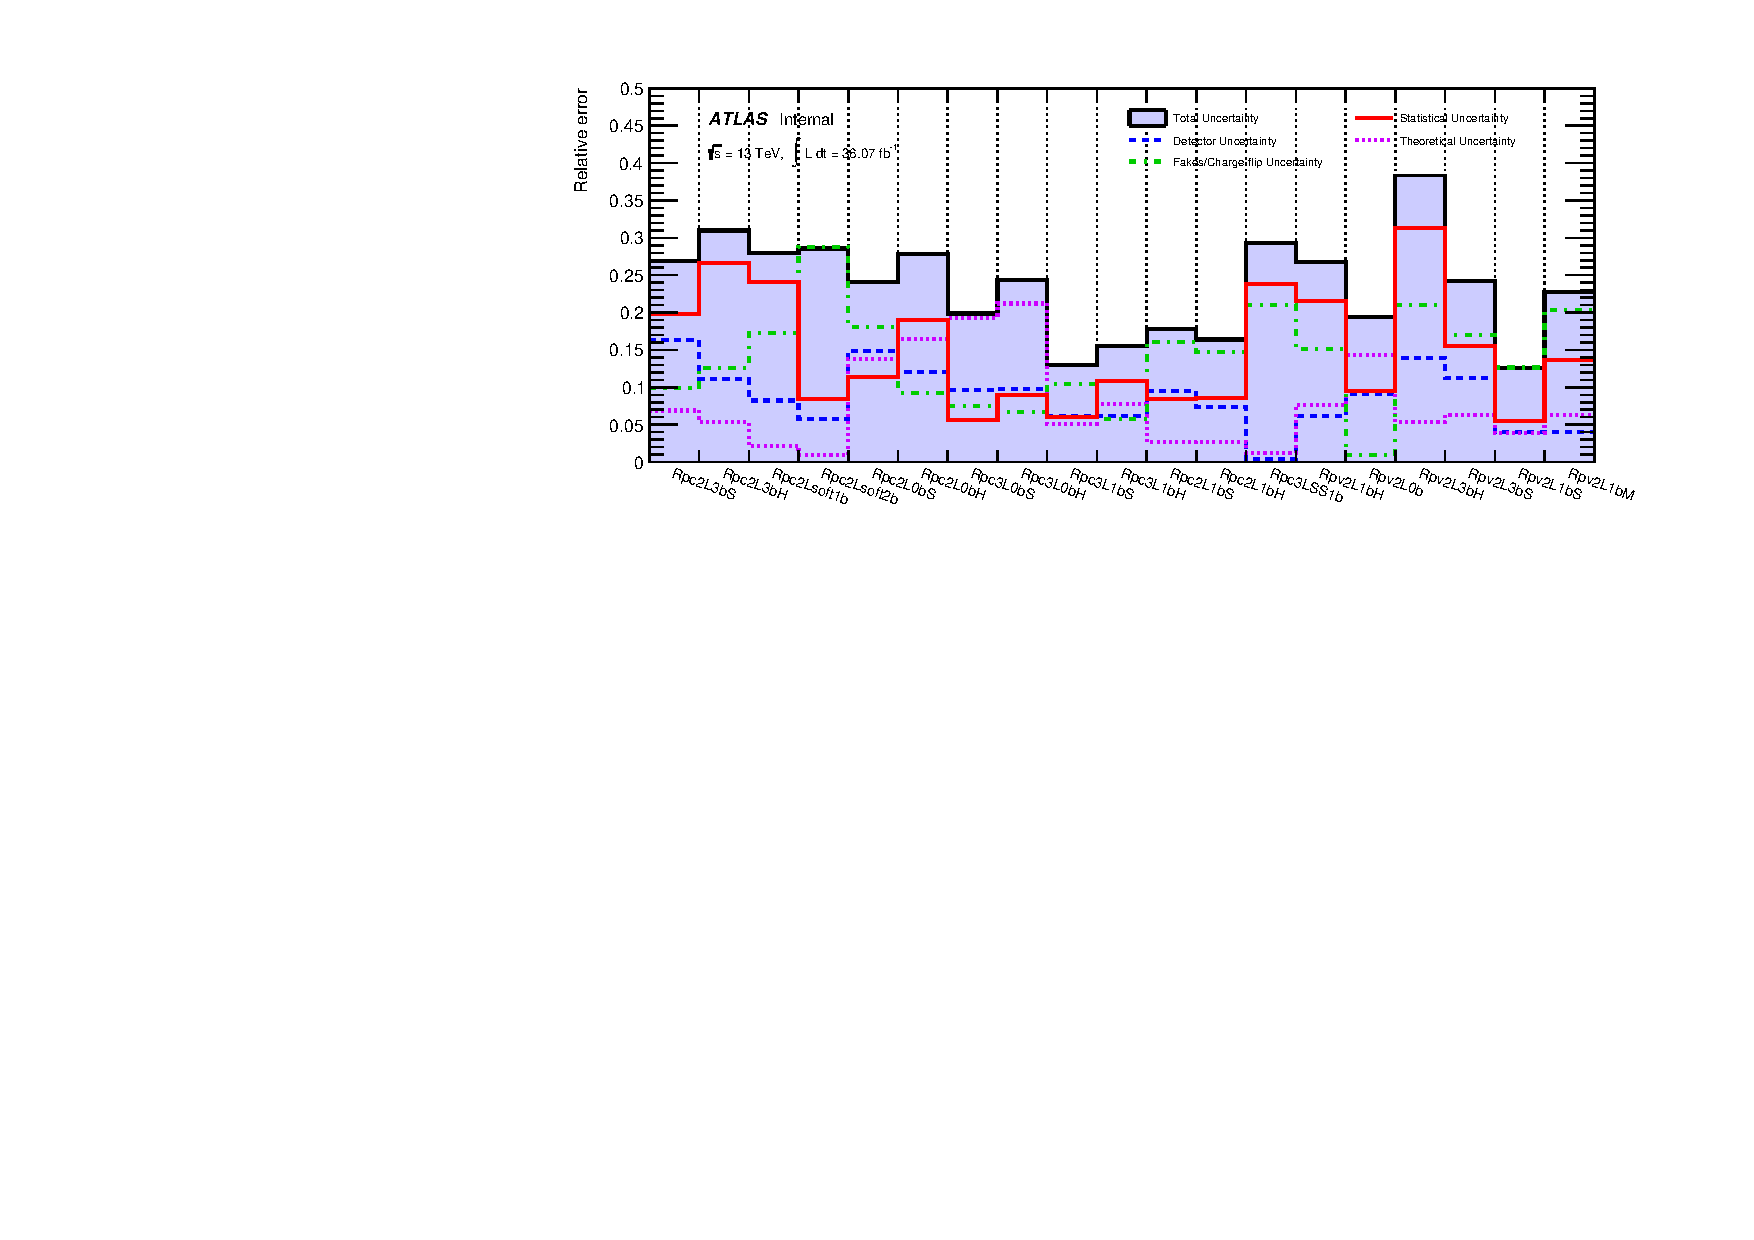
\includegraphics[width=\textwidth]{SystematicsSummary}\caption{}\end{subfigure} \\
\begin{subfigure}[t]{0.87\textwidth}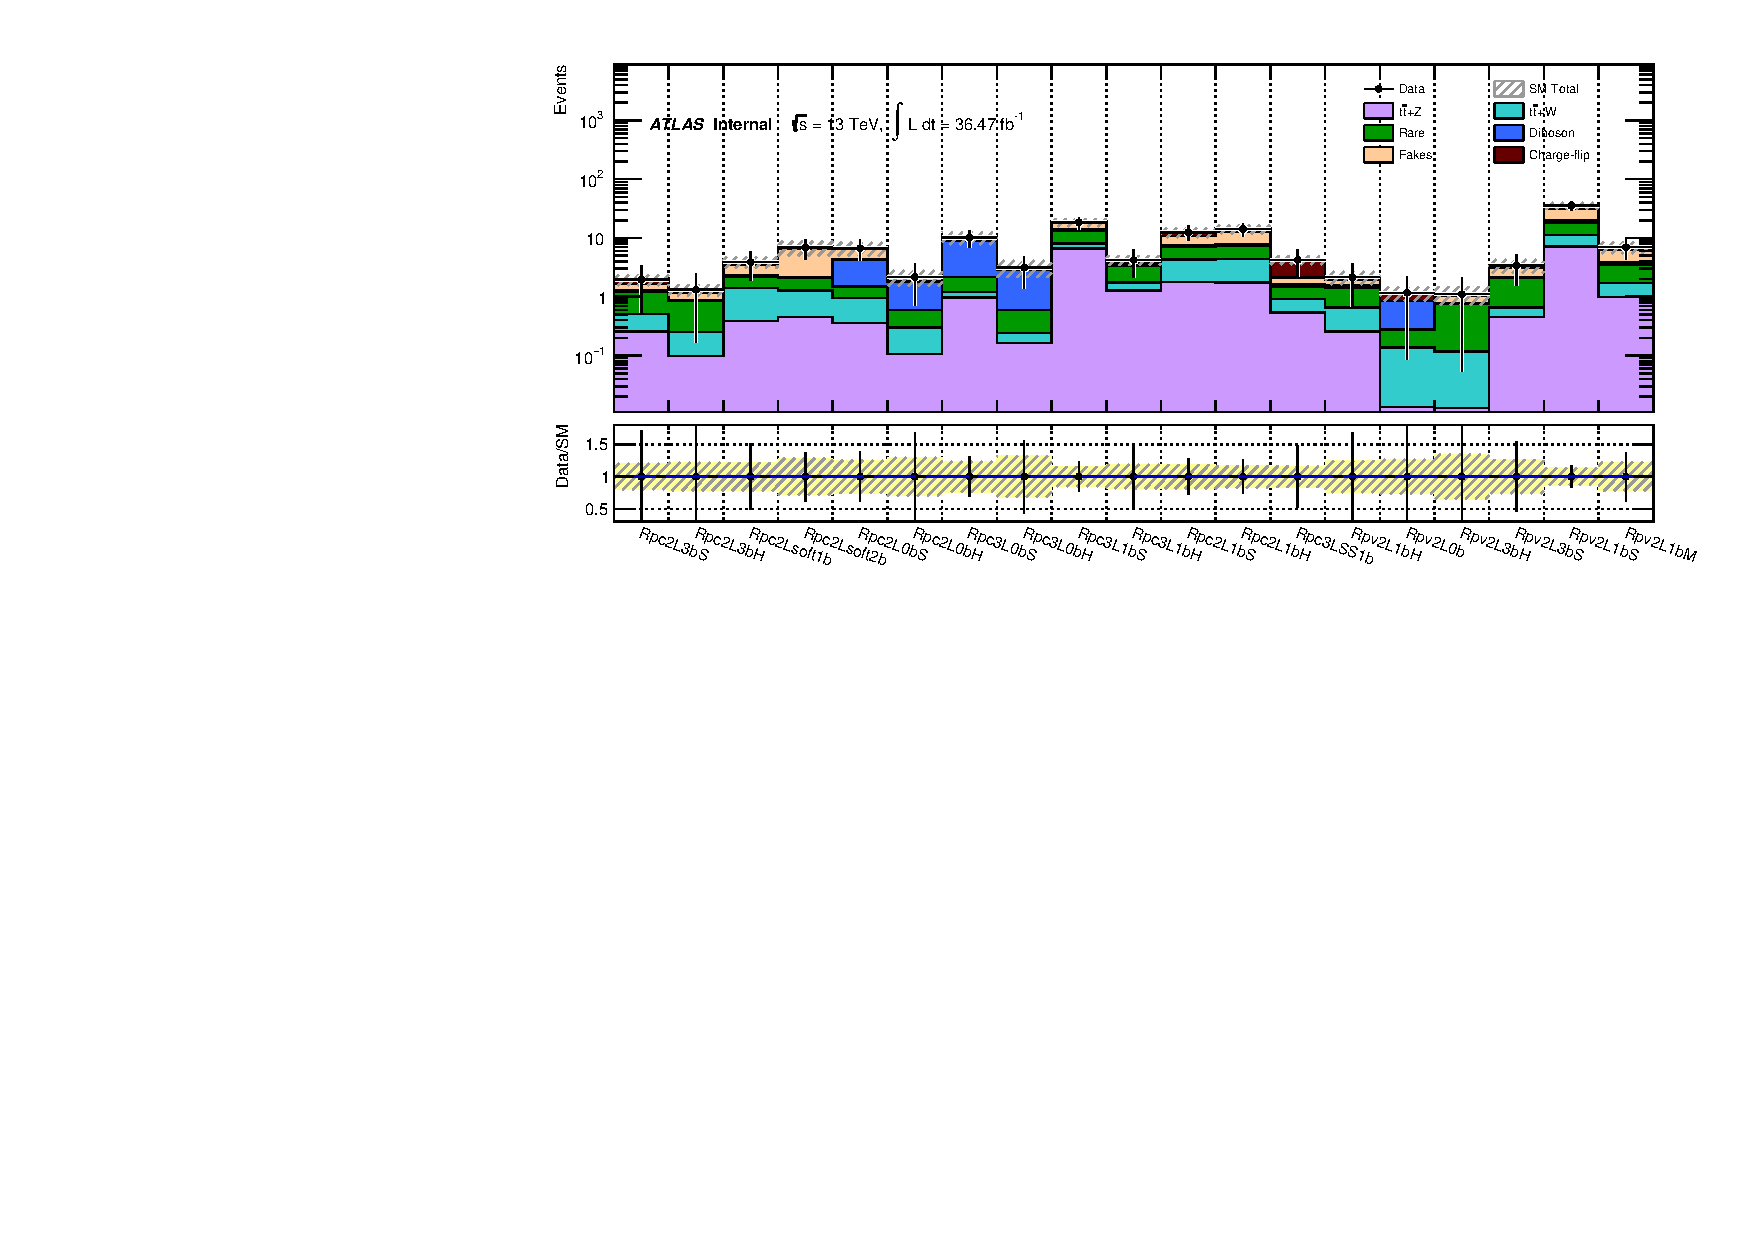
\includegraphics[width=\textwidth]{SRsummary}\caption{}\end{subfigure}
\end{center}
\caption{Relative systematic uncertainties and comparison of the observed and expected event yields in each signal region. 
The background expectations are those obtained from the background-only fits, presented in Table~\ref{tab:SR_yields}. 
\textcolor{red}{[UPDATE: Put all signal regions with final notations. Add ratio plot below SR Event Yields]}} 
\label{fig:PlotSR}
\end{figure}

%\begin{table}[h!]
%\begin{center}
%\caption{The main sources of systematic uncertainty on the SM background estimates for the four signal regions are shown 
%and their values given as relative uncertainties in the expected signal region background event yields. 
%The individual components can be correlated and therefore do not necessarily add up in quadrature to the total systematic uncertainty.
%For reference, the total number of expected background events is also shown.
%}
%\label{tab:SR_syst}
%{\small
%\begin{tabular}{lrrrr}
%\noalign{\smallskip}\hline\hline\noalign{\smallskip}
%         & SR0b3j         & SR0b5j     & SR1b & SR3b     \\[-0.05cm]
%\noalign{\smallskip}\hline\hline\noalign{\smallskip}
%Diboson theoretical uncertainties    & 23\%  &  16\%   &  1\%  &$<$1\%   \\
%$\ttbar V$ theoretical uncertainties & 3\%   &  4\%    & 13\%  &  9\%   \\
%Other theoretical uncertainties      & 5\%   &  3\%    &  9\%  & 15\%   \\
%\noalign{\smallskip}\hline\noalign{\smallskip}
%MC statistical uncertainties         & 11\%  &  14\%   &  3\%  &  6\%   \\
%\noalign{\smallskip}\hline\noalign{\smallskip}
%Jet energy scale        & 12\%   &  11\%  & 6\%    & 5\%   \\
%Jet energy resolution   & 3\%    &  9\%   & 2\%    & 3\%   \\
%$b$-tagging             & 4\%    &  6\%   & 3\%    & 10\%   \\
%PDF                     & 6\%    &  6\%   & 6\%    & 8\%   \\
%Fake/non-prompt leptons & 18\%    &  20\%   & 18\%   & 21\%   \\
%Charge flip             & --     & 1\% & 3\%    & 8\%   \\
%\noalign{\smallskip}\hline\noalign{\smallskip}
%Total background uncertainties & 30\%   & 34\%   & 22\%   & 31\%   \\
%\noalign{\smallskip}\hline\hline\noalign{\smallskip}
%Total background events & $1.5$ & $0.88$ & $4.5$ & $0.80$\\
%\noalign{\smallskip}\hline\hline\noalign{\smallskip}
%\end{tabular}
%}
%\end{center}
%\end{table}
	


%-------------------------------------------------------------------------------
\section{Results, interpretation and limits}
\label{sec:result}
%-------------------------------------------------------------------------------

\begin{table}[htb!]
\begin{center}
\setlength{\tabcolsep}{0.0pc}
\caption{The number of observed data events and expected background contributions in the signal regions. 
The $p$-value of the observed events for the background-only hypothesis is denoted by $p(s = 0)$. 
The ``Rare'' category contains the contributions from associated production of $\ttbar$ with $h/WW/t/\ttbar$, 
as well as $tZ$, $Wh$, $Zh$, and triboson production. 
Background categories shown as ``$-$'' denote that they cannot contribute to a given region (charge flips or $W^\pm W^\pm jj$ in 3-lepton regions). 
The individual uncertainties can be correlated and therefore do not necessarily add up in quadrature to the total systematic uncertainty. 
}
\label{tab:SR_yields}
{\small
\begin{tabular*}{\textwidth}{@{\extracolsep{\fill}}lcccc}
\noalign{\smallskip}\hline\hline\noalign{\smallskip}
         & SR0b3j         & SR0b5j     & SR1b & SR3b     \\[-0.05cm]
\noalign{\smallskip}\hline\hline\noalign{\smallskip}
Observed events         & $3$     &  $3$  & $7$  & $1$            \\
\noalign{\smallskip}\hline\noalign{\smallskip}
Total background events & $1.5 \pm 0.4$ & $0.88 \pm 0.29$ & $4.5 \pm 1.0$ & $0.80 \pm 0.25$\\
$p(s = 0)$                &  0.13  &  0.04  &  0.15  &   0.36   \\
\noalign{\smallskip}\hline\noalign{\smallskip}
Fake/non-prompt leptons & $<0.2$ & $0.05\pm 0.18$ & $0.8 \pm 0.8$ & $0.13 \pm 0.17$\\
Charge-flip & $-$ & $0.02 \pm 0.01$ & $0.60 \pm 0.12$ & $0.19 \pm 0.06$\\
$t\bar{t}W$ & $0.02 \pm 0.01$ & $0.08 \pm 0.04$ & $1.1 \pm 0.4$ & $0.10 \pm 0.05$\\
$t\bar{t}Z$ & $0.10 \pm 0.04$ & $0.05 \pm 0.03$ & $0.92 \pm 0.31$ & $0.14 \pm 0.06$\\
$WZ$ & $1.2 \pm 0.4$ & $0.48 \pm 0.20$ & $0.18 \pm 0.11$ & $<0.02$\\
$W^\pm W^\pm jj$ & $-$ & $0.12 \pm 0.07$ & $0.03 \pm 0.02$ & $<0.01$\\
$ZZ$ & $<0.03$ & $<0.04$ & $<0.03$ & $<0.03$\\
Rare & $0.14 \pm 0.08$ & $0.07 \pm 0.05$ & $0.8 \pm 0.4$ & $0.24 \pm 0.14$\\  
\noalign{\smallskip}\hline\hline\noalign{\smallskip}
\end{tabular*}
}
\end{center}
\end{table}

\begin{figure}[t!]
\centering
\begin{subfigure}[t]{0.49\textwidth}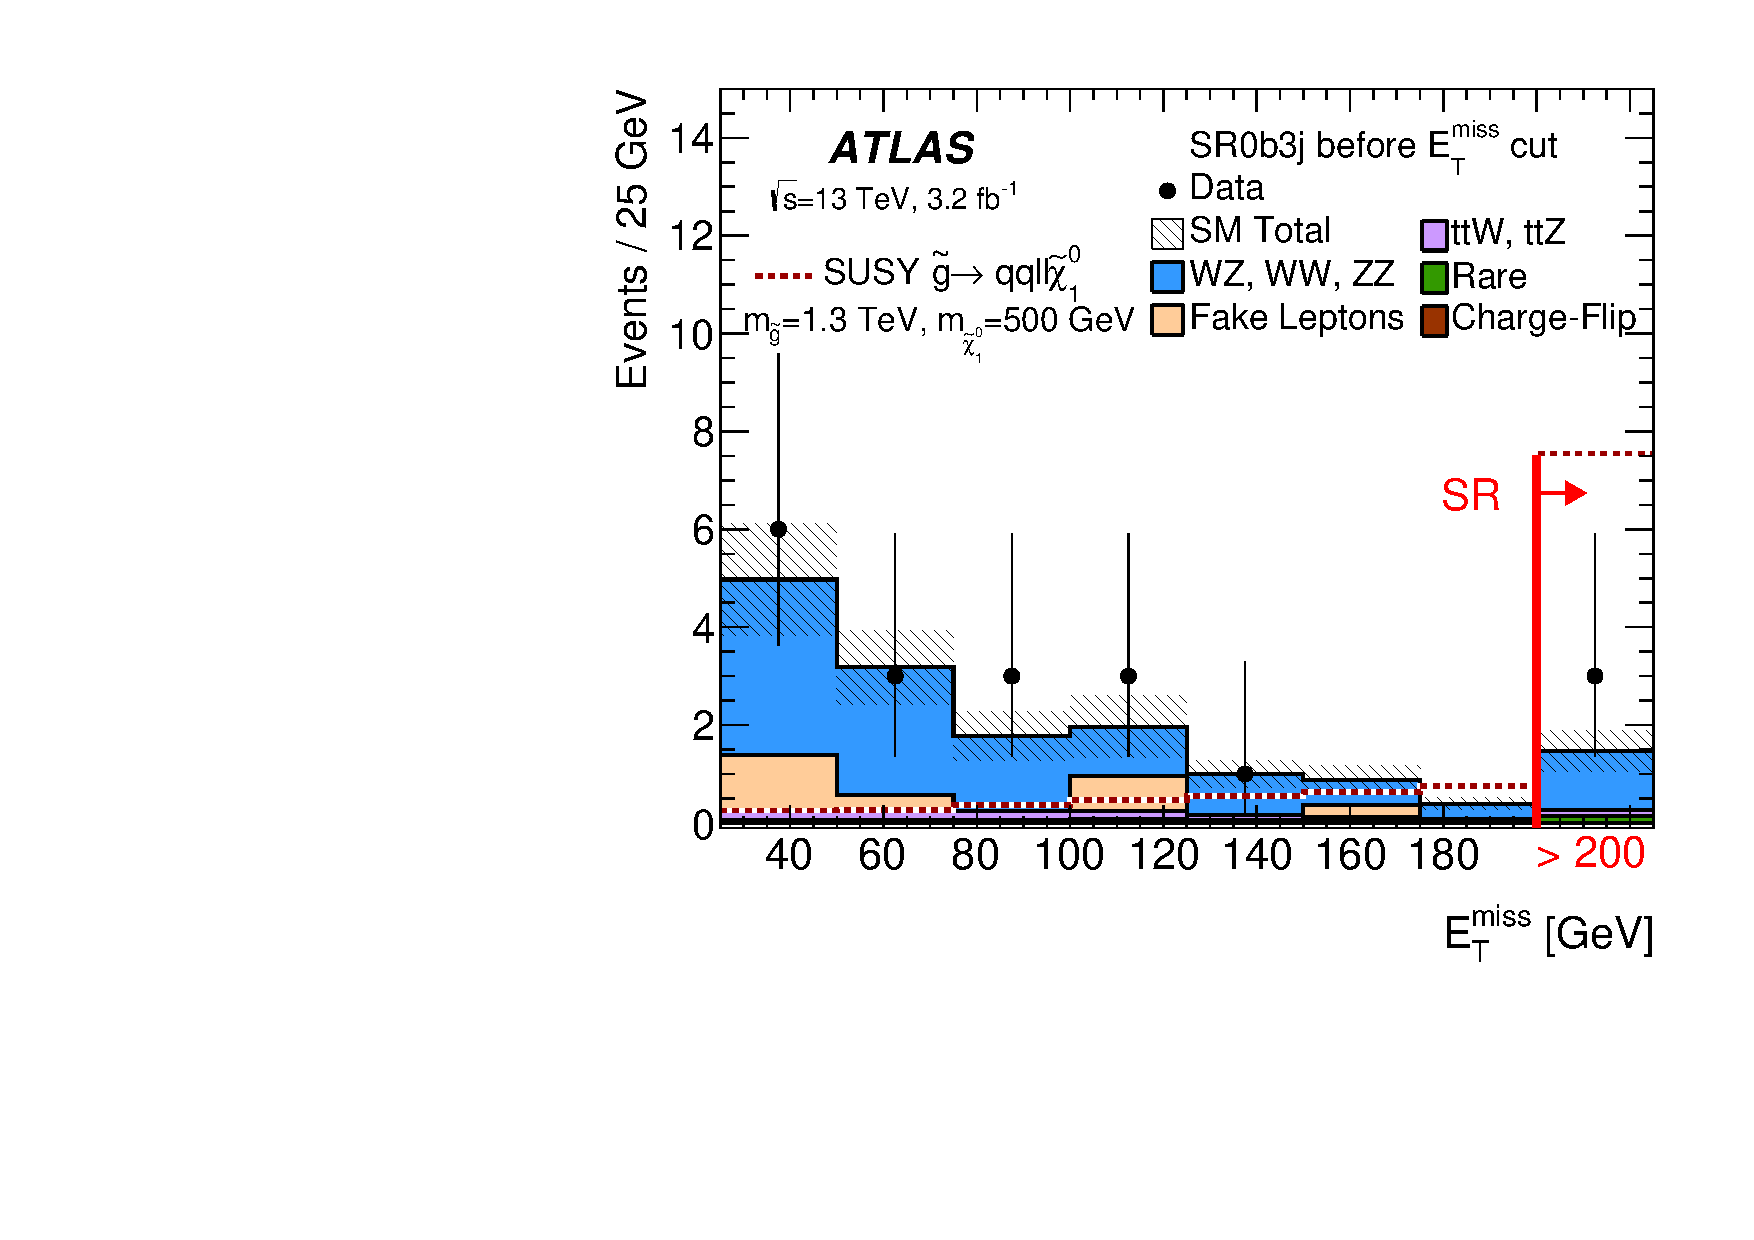
\includegraphics[width=\textwidth]{FIGURES/CONF_SR0b3j.pdf}
\caption{}\label{fig:Results_SR0b3j}\end{subfigure}
\begin{subfigure}[t]{0.49\textwidth}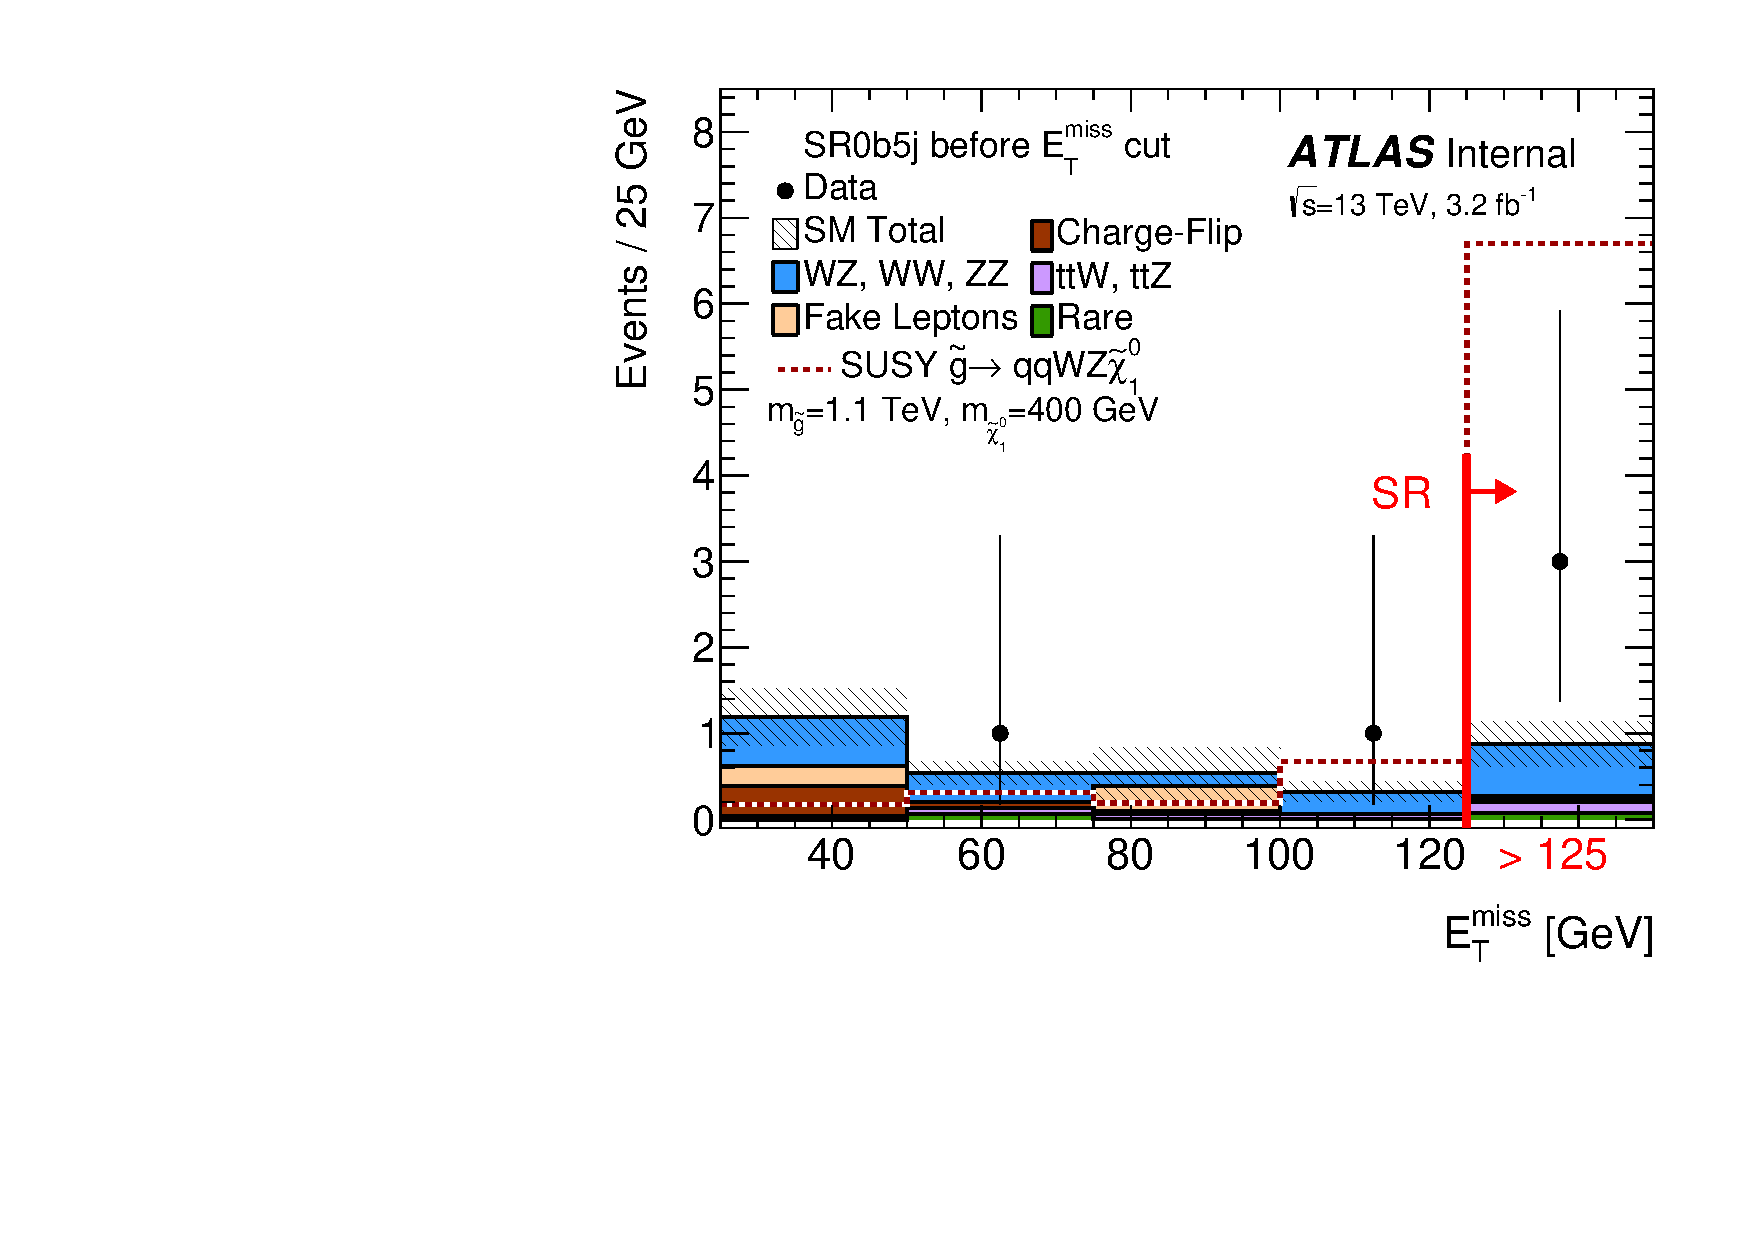
\includegraphics[width=\textwidth]{FIGURES/CONF_SR0b5j.pdf}
\caption{}\label{fig:Results_SR0b5j}\end{subfigure}
\begin{subfigure}[t]{0.49\textwidth}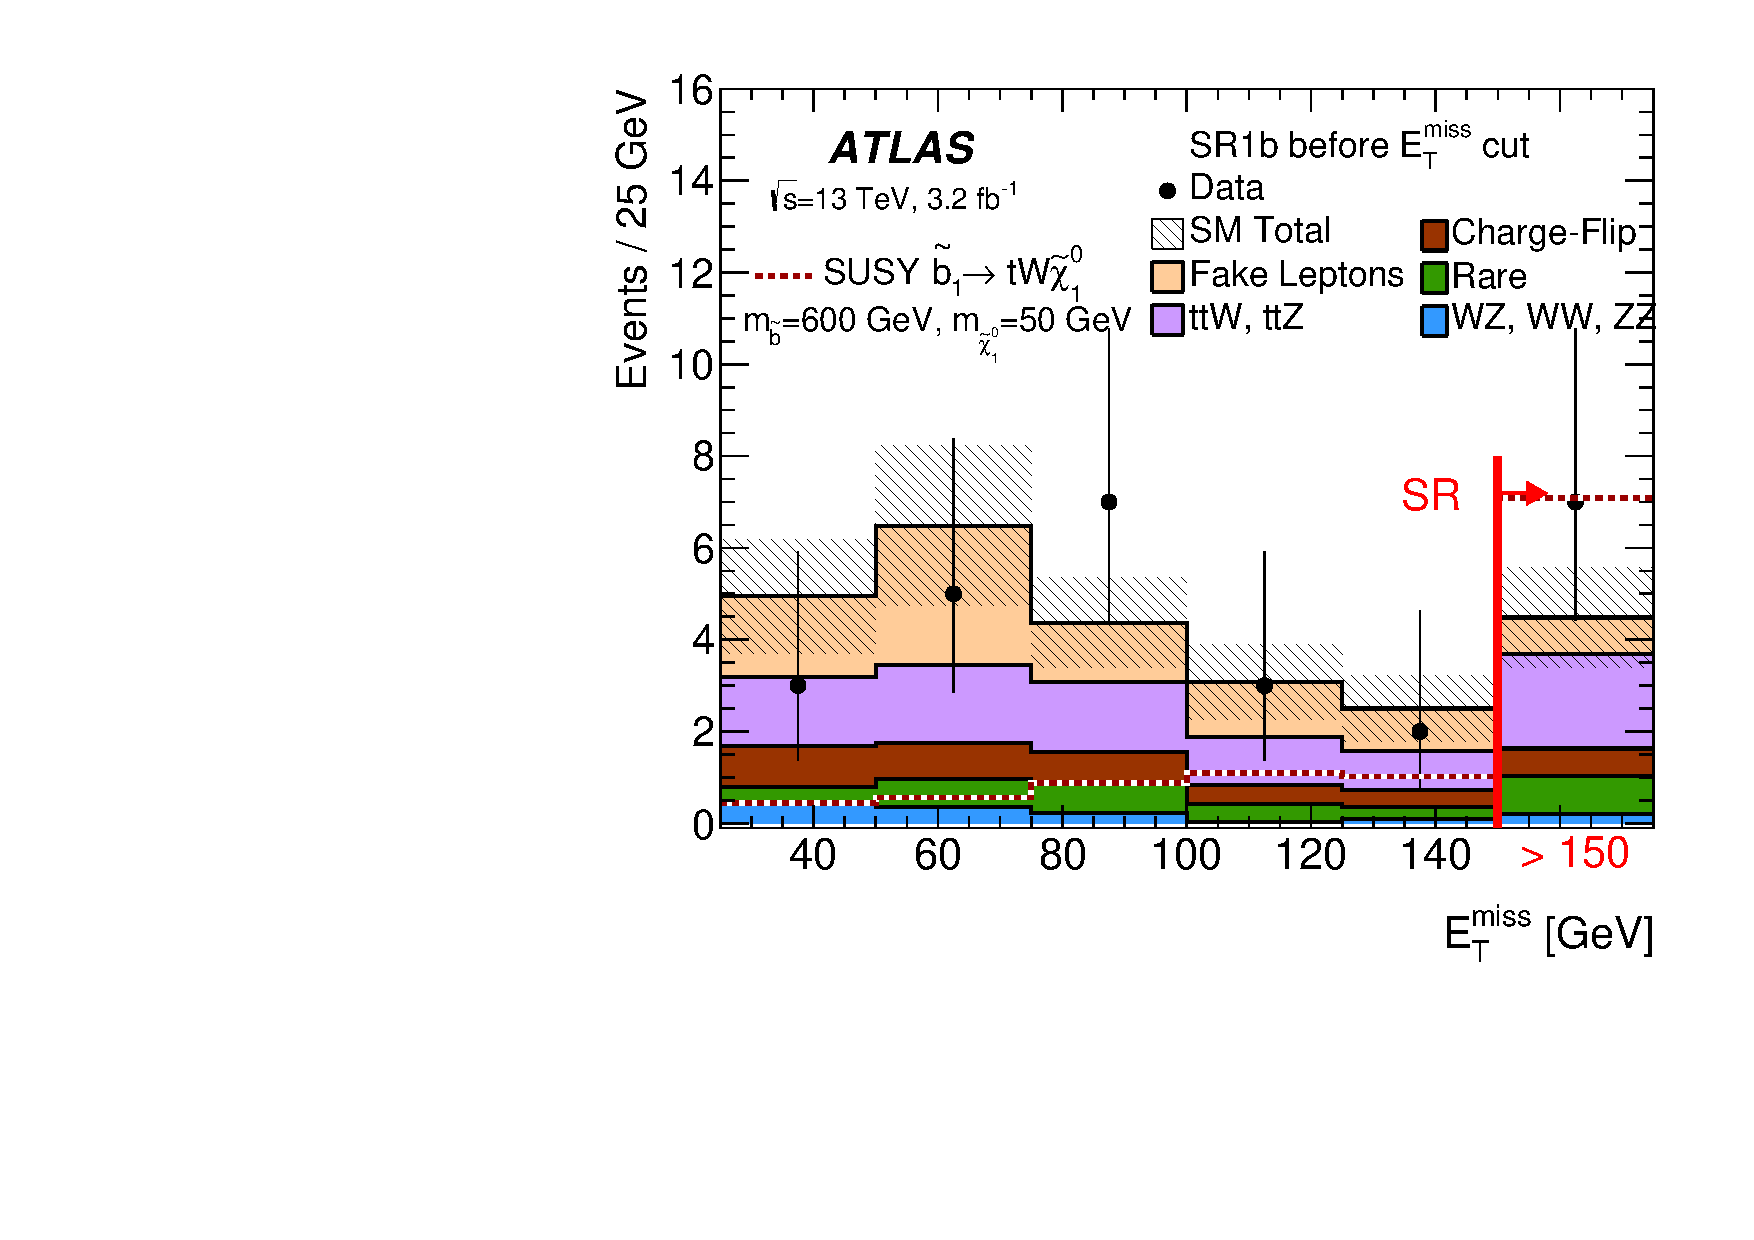
\includegraphics[width=\textwidth]{FIGURES/CONF_SR1b.pdf}
\caption{}\label{fig:Results_SR1b}\end{subfigure}
\begin{subfigure}[t]{0.49\textwidth}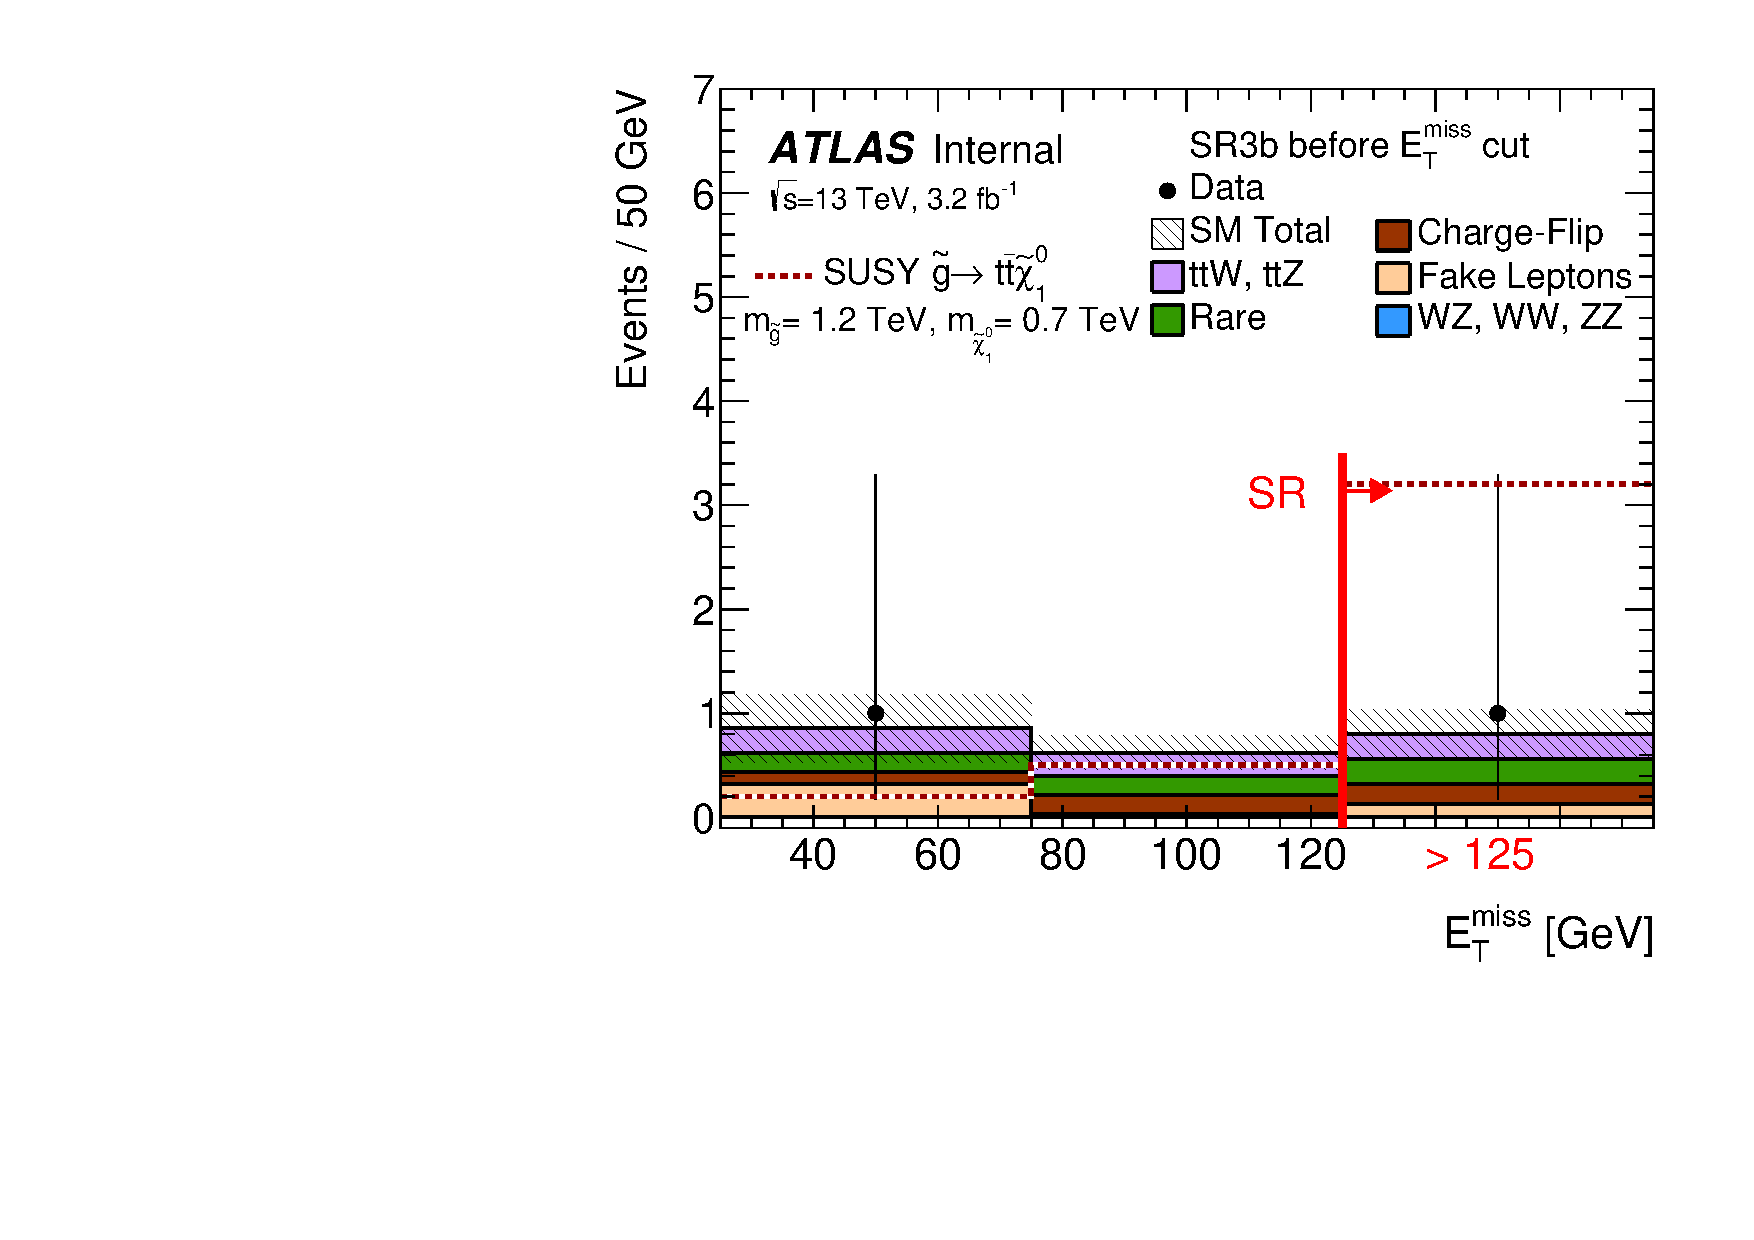
\includegraphics[width=\textwidth]{FIGURES/CONF_SR3b.pdf}
\caption{}\label{fig:Results_SR3b}\end{subfigure}
\caption{Missing transverse momentum distributions after (a) SR0b3j, (b) SR0b5j, (c) SR1b and (d) SR3b selection, beside the \met requirement. 
The results in the signal regions are shown in the last (inclusive) bin of each plot. 
The statistical uncertainties in the background prediction are included in the uncertainty band, 
as well as the theory uncertainties for the backgrounds with prompt SS/3L, 
and the full systematic uncertainties for data-driven backgrounds. 
The ``Fake leptons'' category corresponds to FNP leptons (see text), 
and the ``Rare'' category contains the contributions from associated production of $\ttbar$ with $h/WW/t/\ttbar$, 
as well as $tZ$, $Wh$, $Zh$, and triboson production. 
}
\label{fig:Results_SR_metD} 
\end{figure} 


Figure~\ref{fig:Results_SR_metD} shows the data \met distributions after the signal region selections (beside that on \met) in data 
together with the expected contributions from all the SM backgrounds with their total statistical and systematic uncertainties. 
For illustration, a typical SUSY signal distribution corresponding to the most relevant benchmark scenario 
in each SR is displayed.
The detailed yields for data and the different sources of SM background in the signal regions 
are presented in Table~\ref{tab:SR_yields}. 
The uncertainties amount to 22--34\% of the total background depending on the signal region. 
In all four SRs the number of data events exceeds the expectation but is consistent within the uncertainties, 
the smallest $p$-value for the SM-only hypothesis being 0.04 for SR0b5j. 
Out of the 14 events in the SRs, 2 of the events in SR1b and the 3 events in SR0b3j contain three leptons. 
None of those events contain three leptons of equal charge. 

In the absence of any significant deviations from the SM predictions, upper limits on possible BSM contributions to the signal regions are computed, 
in particular in the context of the SUSY benchmark scenarios described in Section~\ref{sec:intro}. 
The HistFitter framework~\cite{Baak:2014wma}, which utilises a profile-likelihood-ratio test~\cite{Cowan:2010js}, 
is used to establish 95\% confidence intervals using the CL$_\mathrm{s}$ prescription~\cite{Read_CLs}. 
The likelihood is built as the product of a Poisson probability density function describing the observed number of events in the signal region 
and Gaussian distributions constraining the nuisance parameters 
associated with the systematic uncertainties whose widths correspond to the sizes of these uncertainties; 
Poisson distributions are used instead for MC statistical uncertainties. 
Correlations of a given nuisance parameter across the different sources of backgrounds and the signal are taken into account when relevant. 
The statistical tests are performed independently for each of the signal regions. 

Table~\ref{tab:upperlimits} presents 95\% confidence level (CL) model-independent upper limits 
on the number of BSM events, $N_\mathrm{BSM}$, that may contribute to the signal regions. 
Normalising these by the integrated luminosity $L$ of the data sample, they can be interpreted as upper limits on the visible BSM cross-section $\sigma_{\rm{vis}}$, 
defined as the product $\sigma_{\rm{prod}}\times A \times\epsilon=N_\mathrm{BSM}/L$ of production cross-section, acceptance and reconstruction efficiency. 

\begin{table}[htb!]
\centering
\caption{Signal model-independent upper limits on the number of BSM events ($N_{\rm{BSM}}$) 
  and the visible signal cross-section ($\sigma_{\rm{vis}}$) in the four SRs. 
  The numbers (in parentheses) give the observed (expected under the SM hypothesis) 95\% CL upper
  limits. Calculations are performed with pseudo-experiments.
  The $\pm$1$\sigma$ variations on the expected limit due to the statistical and systematic uncertainties in the background prediction are also shown. 
}
\label{tab:upperlimits}
{\small
\renewcommand{\arraystretch}{1.4}
\begin{tabular*}{\textwidth}{@{\extracolsep{\fill}}lrrrr}
\noalign{\smallskip}\hline\hline\noalign{\smallskip}
         & SR0b3j         & SR0b5j     & SR1b & SR3b     \\[-0.05cm]
\noalign{\smallskip}\hline\hline\noalign{\smallskip}
$N_{\rm{BSM}}^{\rm{obs}}$ ($N_{\rm{BSM}}^{\rm{exp}}$) 
 & $5.9$  $({4.1}^{+1.6}_{-0.8})$
 & $6.4$ $({3.6}^{+1.2}_{-1.1})$
 & $8.8$ $({6.0}^{+2.6}_{-1.6})$ 
 & $3.8$ $({3.7}^{+1.1}_{-0.5})$ \\
$\sigma_{\rm{vis}}^{\rm{obs}}$ [fb] & 1.8 & 2.0 & 2.8 & 1.2\\
\noalign{\smallskip}\hline\hline\noalign{\smallskip}
  \end{tabular*}
}
\end{table} 

\begin{figure}[htb!]
\centering
\begin{subfigure}[t]{0.49\textwidth}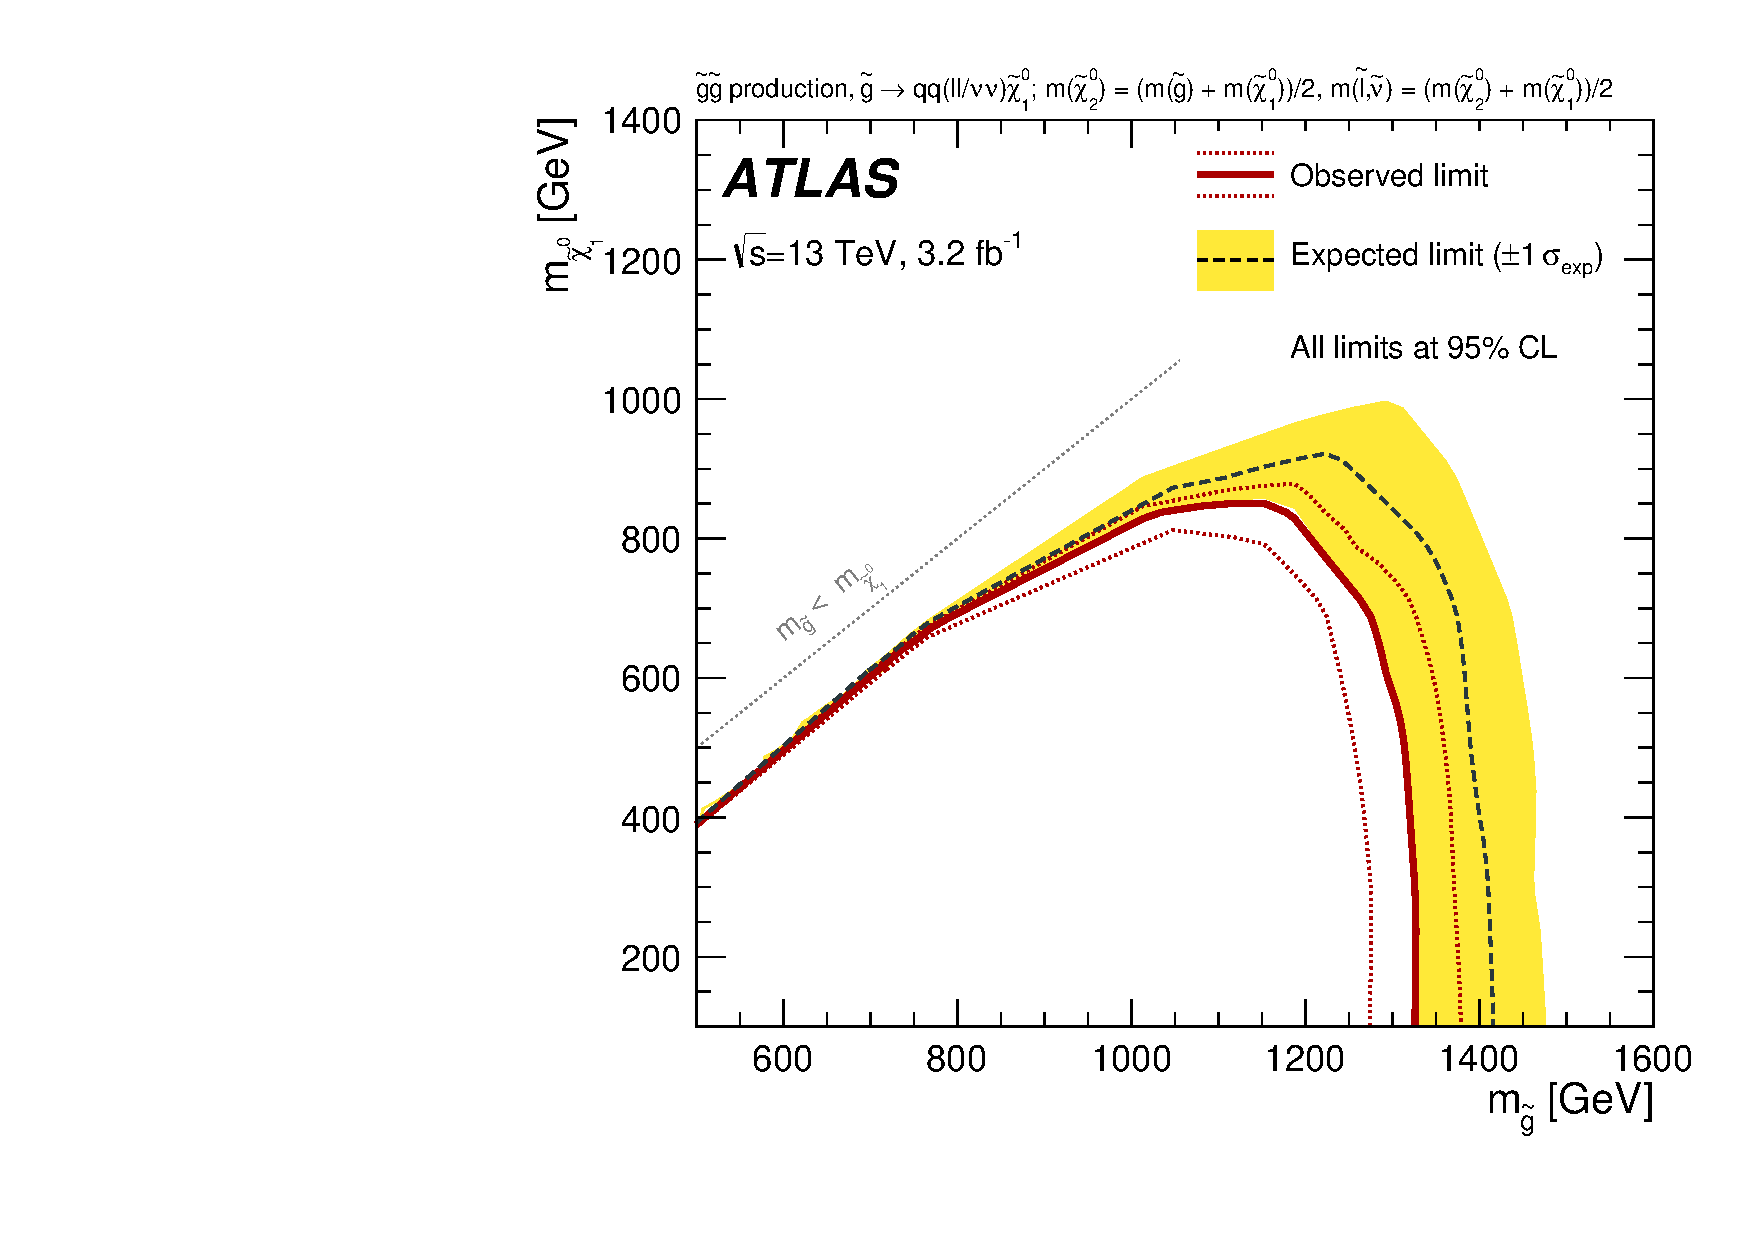
\includegraphics[width=\textwidth]{exclusion2015SameSign_SR0b3j.pdf}
\caption{$\gluino\to q\bar q \ell\ell\ninoone$ scenario, SR0b3j}\label{fig:limits_SR0b3j}\end{subfigure}
\begin{subfigure}[t]{0.49\textwidth}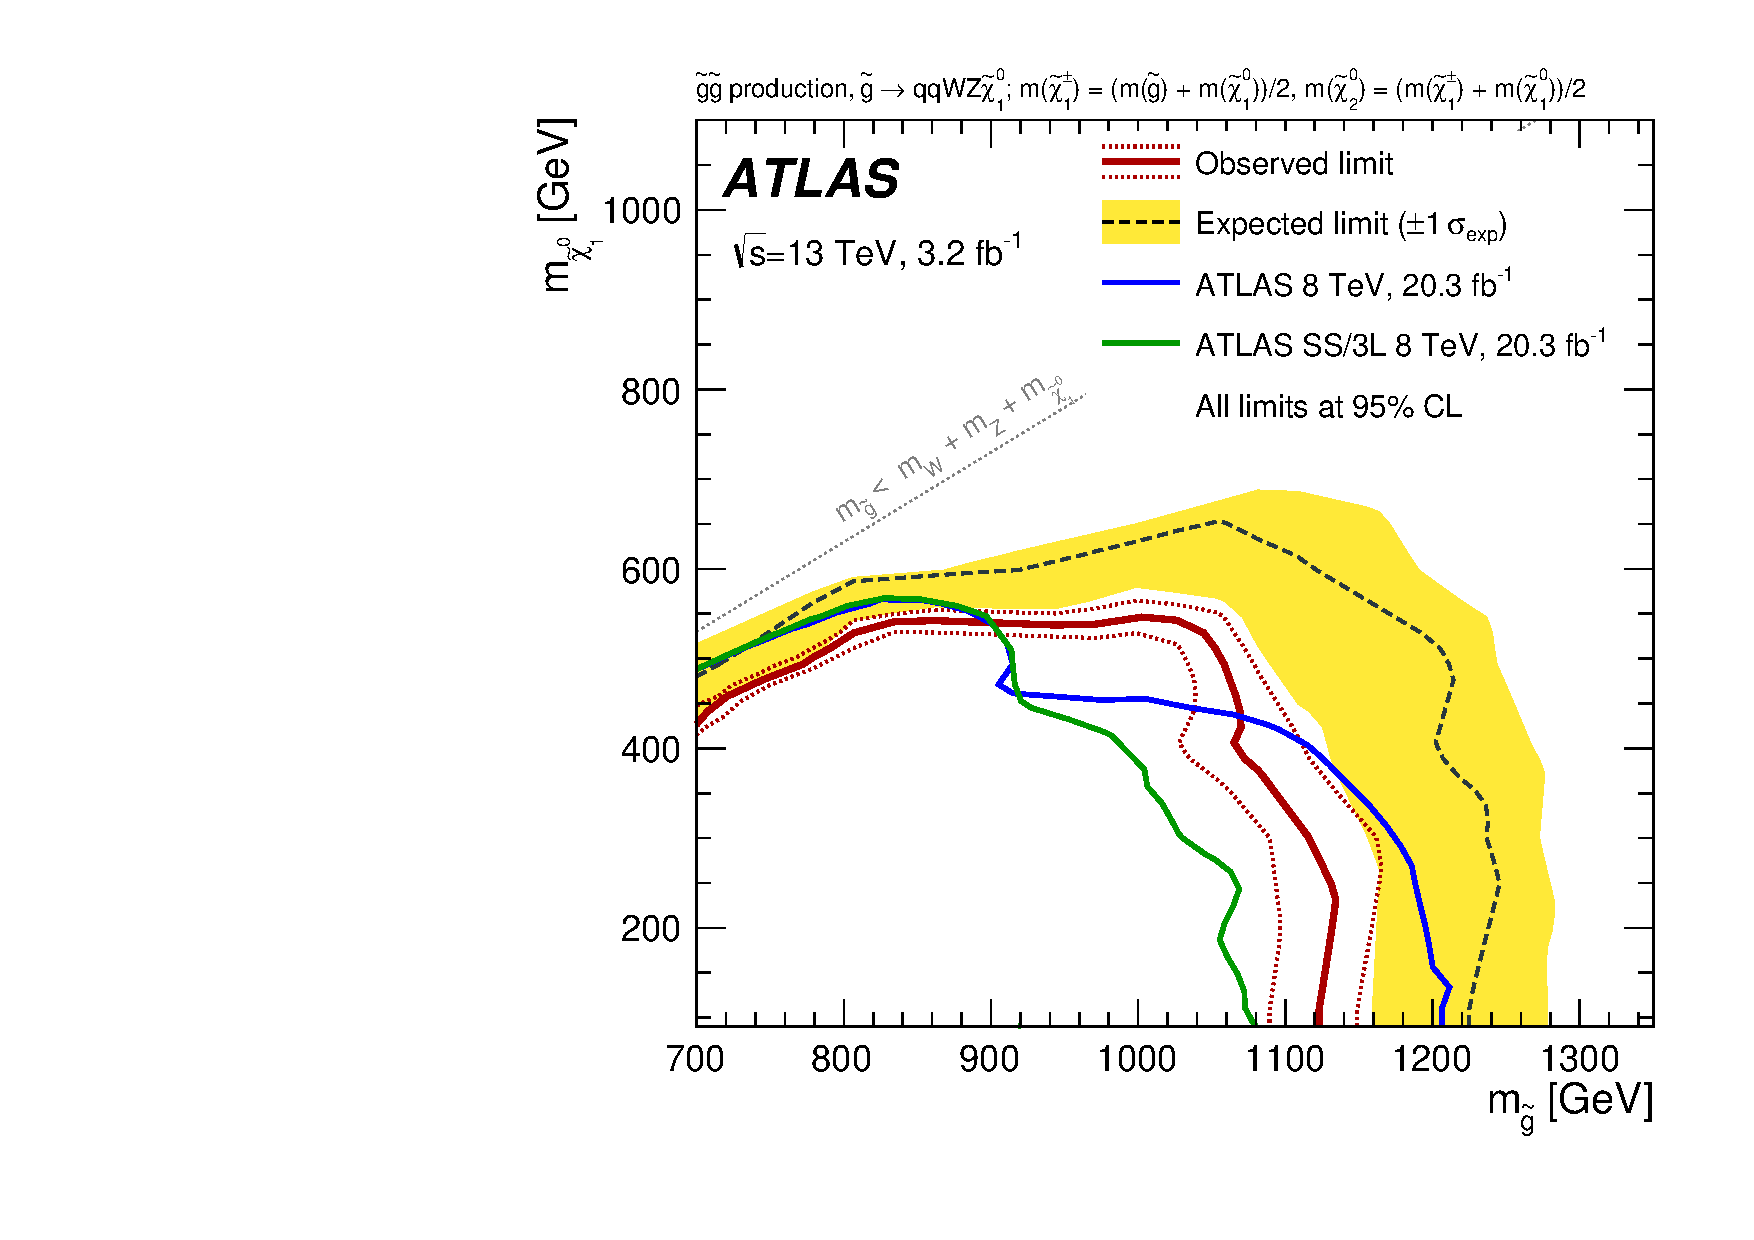
\includegraphics[width=\textwidth]{exclusion2015SameSign_SR0b5j.pdf}
\caption{$\gluino\to q\bar q' WZ\ninoone$ scenario, SR0b5j}\label{fig:limits_SR0b5j}\end{subfigure}
\par\bigskip
\begin{subfigure}[t]{0.49\textwidth}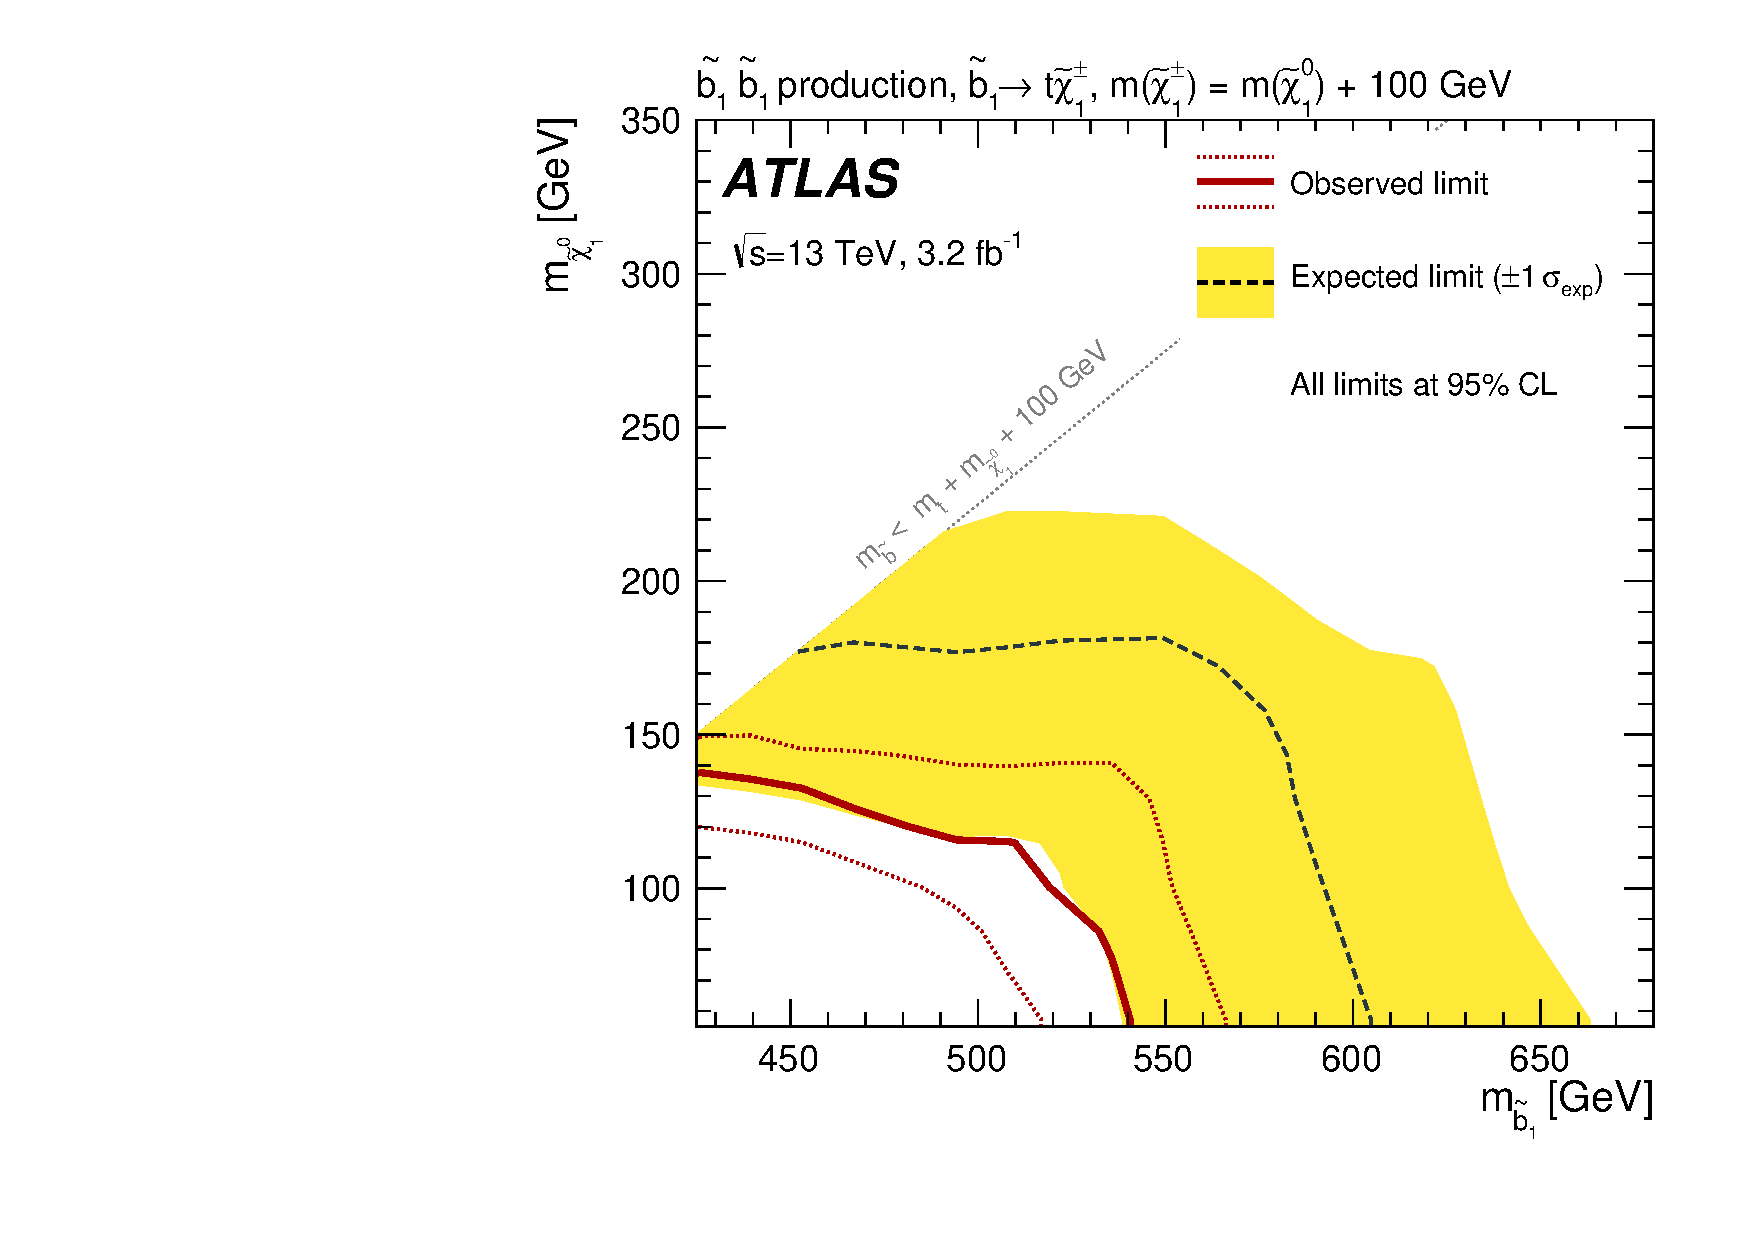
\includegraphics[width=\textwidth]{exclusion2015SameSign_SR1b.pdf}
\caption{$\sbottomone\to tW^-\ninoone$ scenario, SR1b}\label{fig:limits_SR1b}\end{subfigure}
\begin{subfigure}[t]{0.49\textwidth}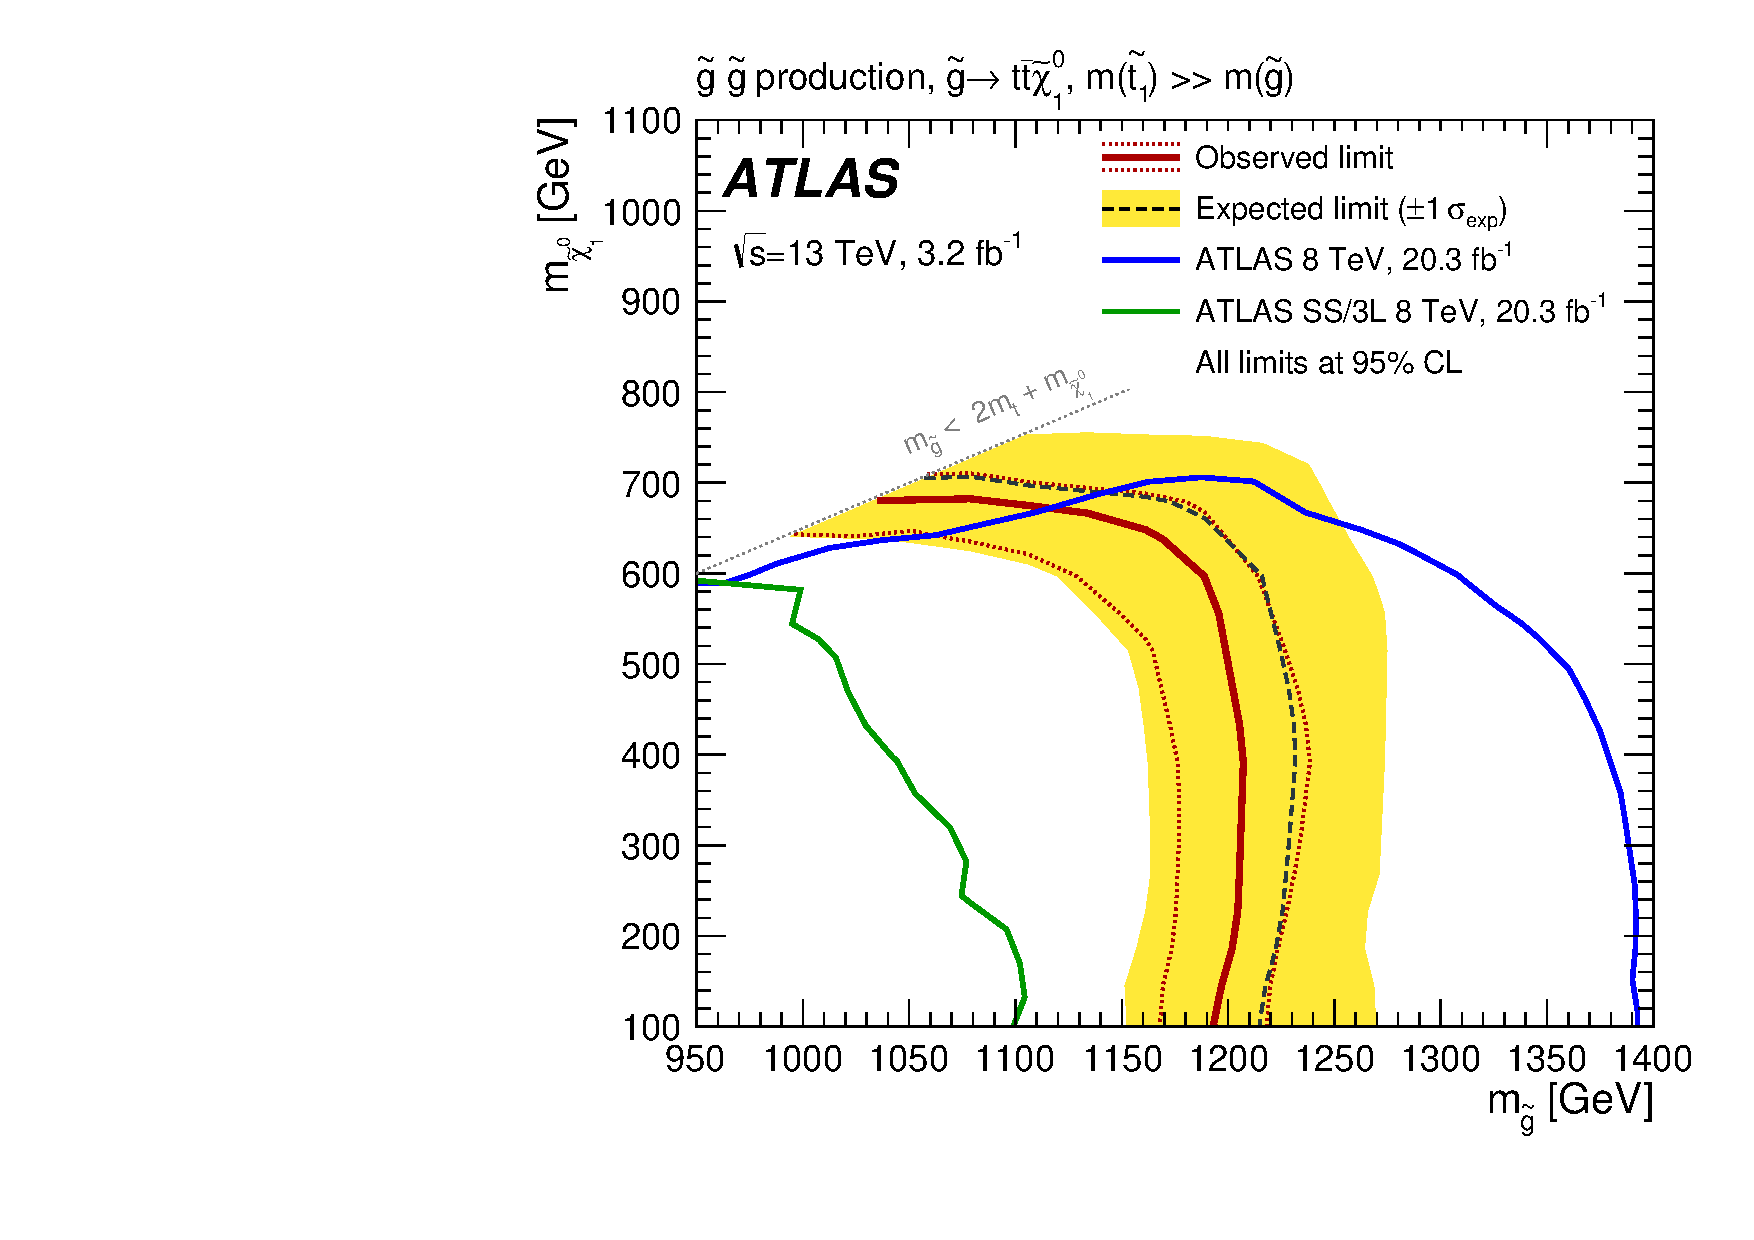
\includegraphics[width=\textwidth]{exclusion2015SameSign_SR3b.pdf}
\caption{$\gluino\to t\bar t\ninoone$ scenario, SR3b}\label{fig:limits_SR3b}\end{subfigure}
\caption{
Observed and expected exclusion limits on the \gluino, \sbottomone and \ninoone masses 
in the context of SUSY scenarios with simplified mass spectra 
featuring $\gluino\gluino$ or $\sbottomone\sbottomonebar$ pair production with exclusive decay modes. 
The signal region used to obtain the limits is specified for each scenario. 
The contours of the band around the expected limit are the $\pm$1$\sigma$ results, 
  including all uncertainties except theoretical uncertainties on the signal cross-section. The dotted lines around the observed
    limit illustrate the change in the observed limit as the nominal signal cross-section is scaled up and down
    by the theoretical uncertainty. All limits are computed at 95\% CL. 
    The diagonal lines indicate the kinematic limit for the decays in each specified scenario.  
For figures (b) and (d), results are compared with the observed limits obtained by previous ATLAS searches~\cite{paperSS3L,Aad:2015iea,Aad:2015pfx}. 
For figures (a) and (c), a direct comparison with earlier searches is not possible, due to differing model assumptions. 
}
\label{fig:Results_Limits} 
\end{figure} 

Exclusion limits are also set on the masses of the superpartners involved in the four SUSY benchmark scenarios considered in this analysis. 
Simplified models corresponding to a single production mode and with 100\% branching ratio to a specific decay chain are used, 
with the masses of the SUSY particles not involved in the process set to very high values. 
Figure~\ref{fig:Results_Limits} shows the limits 
on the mass of the $\ninoone$ as a function of the $\gluino$ or $\sbottomone$ mass. 
%For these results, asymptotic formulas~\cite{Cowan:2010js} are used to model the probability distribution of the test statistic. 
In some cases, the new limits set by this analysis can be compared 
with the existing limits set by the combination of ATLAS SUSY searches with 8 TeV data~\cite{Aad:2015iea,Aad:2015pfx}. 
For parts of the parameter space, the sensitivity reached with the 13 TeV dataset exceeds that of the 8 TeV dataset,
and additional parameter space regions can be excluded, especially for large neutralino masses. 

Signal models featuring gluino pair production with a subsequent gluino decay via $\ninotwo$ and light sleptons\\ 
($\gluino\to q\bar q\ninotwo\to q\bar q (\ell\slepton^*/\nu\tilde{\nu}^*)\to q\bar q(\ell^+\ell^-/\nu\nu)\ninoone$) 
are probed using SR0b3j (Fig.~\ref{fig:limits_SR0b3j}).
In this simplified model, the gluinos decay into $u\bar u$, $d\bar d$, $s\bar s$ or $c\bar c$ with equal probabilities, 
and the six types of leptons are also produced in the $\tilde\chi_2^0$ decays with equal probabilities. 
The $\ninotwo$ mass is set to $m_{\ninotwo}=(m_{\gluino} + m_{\ninoone})/2$, 
with the $\slepton$ and $\tilde{\nu}$ masses set to $m_{\slepton,\tilde{\nu}}=(m_{\ninotwo} + m_{\ninoone})/2$.
Gluino masses up to $m_{\gluino}\approx\SI{1.3}{TeV}$ for a light \ninoone and \ninoone masses up to $m_{\ninoone}\approx\SI{850}{GeV}$ for gluinos with $m_{\gluino}\approx\SI{1.1}{TeV}$ are excluded in this scenario. 

Similarly, models with gluino production  with a subsequent two-step gluino decay via $\chinoonepm$ and $\ninotwo$\\ 
($\gluino\to q\bar q \chinoonepm \to q\bar q W\ninotwo \to  q\bar q W Z \ninoone$) 
are probed with SR0b5j (Fig.~\ref{fig:limits_SR0b5j}).
In this simplified model, the gluinos decay into $u\bar u$, $d\bar d$, $s\bar s$ or $c\bar c$ with equal probabilities. 
The $\chinoonepm$ mass is set to $m_{\chinoonepm}=(m_{\gluino} + m_{\ninoone})/2$ and
the $\ninotwo$ mass is set to $m_{\ninotwo}=(m_{\chinoonepm} + m_{\ninoone})/2$; 
$W$ and $Z$ bosons produced in the decay chain are not necessarily on-shell. 
The exclusion limits in this scenario reach $m_{\gluino}\approx\SI{1.1}{TeV}$ (for light $\ninoone$) and $m_{\ninoone}\approx\SI{550}{GeV}$ (for $m_{\gluino}\approx\SI{1.0}{TeV}$).

Exclusion limits in a simplified model of bottom squark production with chargino-mediated $\sbottomone\to tW^-\ninoone$ decays are 
obtained with SR1b (Fig.~\ref{fig:limits_SR1b}).
In this model the $\chinoonepm$ mass is set to $m_{\chinoonepm}=m_{\ninoone} + \SI{100}{GeV}$.
The limits can reach mass values of $m_{\sbottomone}\approx\SI{540}{GeV}$ for a light $\ninoone$, 
while $m_{\ninoone}\lesssim\SI{140}{GeV}$ are also excluded for $m_{\sbottomone}\approx\SI{425}{GeV}$, 
significantly extending the previous limits obtained at $\sqrt{s}=8$~TeV~\cite{Aad:2015pfx} 
which excluded $m_{\sbottomone}\lesssim\SI{470}{GeV}$ for $m_{\ninoone}\approx\SI{60}{GeV}$ for a similar model.

Finally, SR3b is used to set limits on masses in a simplified model with 
gluino pair production and $\gluino\to t\bar t\ninoone$ decays 
via an off-shell top squark (Fig.~\ref{fig:limits_SR3b}). 
In that case, gluino masses of $m_{\gluino}\lesssim\SI{1.2}{TeV}$ are excluded for $m_{\ninoone}\lesssim\SI{600}{GeV}$, 
and $\ninoone$ masses up to $m_{\ninoone}\approx\SI{680}{GeV}$ are also excluded for $m_{\gluino}\approx\SI{1.05}{TeV}$. 


\FloatBarrier

%-------------------------------------------------------------------------------
\section{Conclusion}
\label{sec:conclusion}
%-------------------------------------------------------------------------------

A search for supersymmetry in events with exactly two same-sign leptons or at least three leptons, multiple jets, 
$b$-jets and large $\met$ and/or $\meff$ is presented. 
The analysis is performed with proton--proton collision data at $\sqrt{s}=13\TeV$ 
collected between August 2015 and October 2016 with the ATLAS detector at the Large Hadron Collider 
corresponding to an integrated luminosity of 36.0 fb$^{-1}$. 
With no significant excess over the Standard Model expectation observed,
results are interpreted in the framework of simplified models featuring gluino 
and squark production in $R$-parity conserving and $R$-parity violating scenarios. Upper limits on particle 
masses are derived at 95\% confidence level. 
In the $\gluino\gluino$ simplified models considered, $m_{\gluino}\lesssim$ \textcolor{red}{[UPDATE]}~TeV and $m_{\ninoone}\lesssim$\textcolor{red}{[UPDATE]}~TeV 
are excluded depending on the model parameters. 
Bottom squark masses of $m_{\sbottomone}\lesssim$ \textcolor{red}{[UPDATE]}~GeV
are also excluded for a light $\ninoone$ in a $\sbottomone\sbottomonebar$ simplified model with $\sbottomone\to tW^-\ninoone$. 
Masses of right-handed down squark are probed up to $m_{\tilde d_R}\approx$\textcolor{red}{[UPDATE]}~GeV in RPV scenarios. 
Within the models considered, exclusion limits are extended by \textcolor{red}{[UPDATE]}~GeV in $\gluino$ mass, 
\textcolor{red}{[UPDATE]}~GeV in $\ninoone$ mass and \textcolor{red}{[UPDATE]}~GeV in $\sbottomone$ mass with respect to previous results.
\textcolor{red}{UPDATE: Add model independent limits on the x-sec of a possible signal contribution to the SRs are set of upto XXX fb.}

%-------------------------------------------------------------------------------
%\section*{Acknowledgements}
%-------------------------------------------------------------------------------
%% Acknowledgements for papers with collision data
% Version 7-Feb-2016

% Standard acknowledgements start here
%----------------------------------------------
We thank CERN for the very successful operation of the LHC, as well as the
support staff from our institutions without whom ATLAS could not be
operated efficiently.

We acknowledge the support of ANPCyT, Argentina; YerPhI, Armenia; ARC, Australia; BMWFW and FWF, Austria; ANAS, Azerbaijan; SSTC, Belarus; CNPq and FAPESP, Brazil; NSERC, NRC and CFI, Canada; CERN; CONICYT, Chile; CAS, MOST and NSFC, China; COLCIENCIAS, Colombia; MSMT CR, MPO CR and VSC CR, Czech Republic; DNRF and DNSRC, Denmark; IN2P3-CNRS, CEA-DSM/IRFU, France; GNSF, Georgia; BMBF, HGF, and MPG, Germany; GSRT, Greece; RGC, Hong Kong SAR, China; ISF, I-CORE and Benoziyo Center, Israel; INFN, Italy; MEXT and JSPS, Japan; CNRST, Morocco; FOM and NWO, Netherlands; RCN, Norway; MNiSW and NCN, Poland; FCT, Portugal; MNE/IFA, Romania; MES of Russia and NRC KI, Russian Federation; JINR; MESTD, Serbia; MSSR, Slovakia; ARRS and MIZ\v{S}, Slovenia; DST/NRF, South Africa; MINECO, Spain; SRC and Wallenberg Foundation, Sweden; SERI, SNSF and Cantons of Bern and Geneva, Switzerland; MOST, Taiwan; TAEK, Turkey; STFC, United Kingdom; DOE and NSF, United States of America. In addition, individual groups and members have received support from BCKDF, the Canada Council, CANARIE, CRC, Compute Canada, FQRNT, and the Ontario Innovation Trust, Canada; EPLANET, ERC, FP7, Horizon 2020 and Marie Sk{\l}odowska-Curie Actions, European Union; Investissements d'Avenir Labex and Idex, ANR, R{\'e}gion Auvergne and Fondation Partager le Savoir, France; DFG and AvH Foundation, Germany; Herakleitos, Thales and Aristeia programmes co-financed by EU-ESF and the Greek NSRF; BSF, GIF and Minerva, Israel; BRF, Norway; the Royal Society and Leverhulme Trust, United Kingdom.

The crucial computing support from all WLCG partners is acknowledged
gratefully, in particular from CERN and the ATLAS Tier-1 facilities at
TRIUMF (Canada), NDGF (Denmark, Norway, Sweden), CC-IN2P3 (France),
KIT/GridKA (Germany), INFN-CNAF (Italy), NL-T1 (Netherlands), PIC (Spain),
ASGC (Taiwan), RAL (UK) and BNL (USA) and in the Tier-2 facilities
worldwide.
%----------------------------------------------





%-------------------------------------------------------------------------------
% If you use biblatex and either biber or bibtex to process the bibliography
% just say \printbibliography here
\printbibliography
% If you want to use the traditional BibTeX you need to use the syntax below.
%\bibliographystyle{bibtex/bst/atlasBibStyleWoTitle}
%\bibliography{ss3l2016conf,bibtex/bib/ATLAS}
%-------------------------------------------------------------------------------


%%-------------------------------------------------------------------------------
\clearpage
\appendix
\part*{Appendix}
\addcontentsline{toc}{part}{Appendix}
%%-------------------------------------------------------------------------------
%replaced \ninoone with \tilde\chi^0_1

\begin{figure}[htb!!]
  \begin{center}
 
\includegraphics[width=0.49\textwidth]{figures/Null}
 
\includegraphics[width=0.49\textwidth]{figures/Null}
 \end{center}
  \vspace{-0.8cm}
  \caption{Illustration of the best expected signal region per signal grid point for the $\gluino\to q\bar q (\ell\ell/\nu\nu)\tilde\chi^0_1$ (left) and $\gluino\to q\bar q' WZ\tilde\chi^0_1$ (right) models. This mapping is used for the final combined exclusion limits.}
  \label{fig:stop2_SR}
\end{figure}

\begin{table}[h!]
\centering
\begin{tabular}{|l|rc|}
\hline\hline
& Raw events & \begin{tabular}{@{}c@{}}Number of events expected\\ for 36.0fb$^{-1}$\end{tabular}\\
\hline\hline
\multicolumn{3}{|l|}{XXX, $\gluino\to q\bar q(\ell\ell/\nu\nu)\tilde\chi^0_1$, $m_{\gluino}=\SI{1.4}{TeV}$, $m_{\tilde\chi^0_1}=\SI{1.1}{TeV}$} \\ \hline
produced					& 	   & $--$ \\
$\ge 3$ leptons ($\pt>20,20,\SI{10}{GeV}$)	&  	   & $-- \pm --$\hspace*{1.95mm} \\
trigger						&  	   & $-- \pm --$\hspace*{1.95mm} \\
no $b$-jet ($\pt>\SI{20}{GeV}$)			&  	   & $-- \pm --$\hspace*{1.95mm} \\
$\ge 4$ jets ($\pt>\SI{40}{GeV}$)		&  	   & $--\pm --$\hspace*{1.95mm} \\
$\met>\SI{150}{GeV}$				&  	   & $-- \pm --$ \\
\hline\hline
\end{tabular}
\caption{Number of signal events selected at different stages of the Signal region definitions, 
for some of the RPC benchmark scenarios shown on Fig.~\ref{fig:feynman}. 
Only the statistical uncertainties are displayed. }
\label{tab:signal_cutflow_rpc}
\end{table}


\begin{table}[h!]
\centering
\begin{tabular}{|l|rc|}
\hline\hline
\multicolumn{3}{|l|}{XXXX, $\gluino\to tds$, $m_{\gluino}=\SI{1.4}{TeV}$, $m_{\tilde{t}_1}=\SI{600}{GeV}$} \\ \hline
produced					& 	   & $--$ \\
$\ge 3$ leptons ($\pt>20,20,\SI{10}{GeV}$)	&  	   & $-- \pm --$\hspace*{1.95mm} \\
trigger						&  	   & $-- \pm --$\hspace*{1.95mm} \\
$\ge 1$ $b$-jet ($\pt>\SI{20}{GeV}$)			&  	   & $-- \pm --$\hspace*{1.95mm} \\
$\ge 6$ jets ($\pt>\SI{50}{GeV}$)		&  	   & $--\pm --$\hspace*{1.95mm} \\
$\meff>\SI{1.8}{TeV}$				 &	    & $-- \pm --$ \\
\hline\hline
\end{tabular}
\caption{Number of signal events selected at different stages of the RPV SUSY scenario definitions, 
for some of the RPV benchmark scenarios shown on Fig.~\ref{fig:feynman}. 
Only the statistical uncertainties are displayed. }
\label{tab:signal_cutflow_rpv}
\end{table}


%-------------------------------------------------------------------------------
% Print the list of contributors to the analysis
% The argument gives the fraction of the text width used for the names
%-------------------------------------------------------------------------------
%\clearpage
%\PrintAtlasContribute{0.30}

%%-------------------------------------------------------------------------------
%\clearpage
%\appendix
%\part*{Auxiliary material}
%\addcontentsline{toc}{part}{Auxiliary material}
%%-------------------------------------------------------------------------------
%
%In an ATLAS paper, auxiliary plots and tables that are supposed to be made public 
%should be collected in an appendix that has the title \enquote{Auxiliary material}.
%This appendix should be printed after the Bibliography.
%At the end of the paper approval procedure, this information can be split into a separate document
%-- see \texttt{atlas-auxmat.tex}.
%
%In an ATLAS note, use the appendices to include all the technical details of your work
%that are relevant for the ATLAS Collaboration only (e.g.\ dataset details, software release used).
%This information should be printed after the Bibliography.

\end{document}
